\documentclass[]{report}
\usepackage[utf8]{inputenc}
\usepackage{amsmath, amssymb, graphicx}
\usepackage{hhline}
\graphicspath{{images/}}
\usepackage[a4paper, width=150mm, top=25mm, bottom=25mm, bindingoffset=6mm]{geometry}
%\usepackage{geometry}
%\geometry{a4paper,total={170mm,257mm},left=20mm,top=20mm,}

\usepackage{hyperref} %for links in bibliography

\usepackage{fancyhdr}
\pagestyle{fancy}

\usepackage{natbib} % styling references

\usepackage{float} %for anchoring figures

\usepackage{subcaption} % for subtables
\usepackage{adjustbox} % for tables that are too wide

\usepackage{longtable} %tables that span several pages
\usepackage{multirow} % multiple rows/columns in tables

\usepackage{xcolor}

\usepackage{csquotes}

\usepackage[T1]{fontenc}
\usepackage{titlesec, blindtext, color}
\definecolor{gray75}{gray}{0.75}
\newcommand{\hsp}{\hspace{20pt}}
\titleformat{\chapter}[hang]{\Huge\bfseries}{\thechapter\hsp\textcolor{gray75}\hsp}{0pt}{\Huge\bfseries}

\usepackage{afterpage}

% Load the parskip package with skip and indent options
\usepackage[skip=8pt plus1pt, indent=0pt]{parskip}

\newcommand\blankpage{%
    \null
    \thispagestyle{empty}%
    \addtocounter{page}{-1}%
    \newpage}



\begin{document}
\begin{titlepage}
    \begin{center}
        \vspace*{1cm} % leave space between top page and start of text

        
\includegraphics[width=1\textwidth]{images/crest.png}
        
        \textbf{MT5599 Project}

        \vspace{0.5cm}
        Thesis Subtitle

        \vspace{1.5cm}
        \textbf{Elizaveta Abel}

        \vfill

        A thesis is presented for the degree of \\ 
        MMath (Hons) Mathematics.



        School of Mathematics and Statistics \\
        University of St Andrews \\
        Scotland, United Kingdom \\
        March 2023
        
    \end{center}
\end{titlepage}
\tableofcontents
\afterpage{\blankpage}
\pagenumbering{roman}

\chapter*{Acknowledgements}
\pagenumbering{arabic}
%Jack Burns for saving my project countless times.
%Rachel Sippy for being the most supportive supervisor.
%Jennifer Sampson, Peter Koczka for introducing me to NLP.

\chapter*{Declaration}
I certify that this project report has been written by me, is a record of work carried out by me, and is essentially different from work undertaken for any other purpose or assessment.

\chapter*{Abstract}
100-200 words.
\pagenumbering{arabic}

\chapter{Introduction} %W7
\section{Background}

% what is an epi week?

\subsection{Dengue Fever in South America}

Dengue is a viral disease spread through mosquito bites, primarily by \textit{Aedes aegypti} mosquitoes. The person will have no symptoms for most dengue infections, so they will likely never know they were infected, and the infection will never get reported. However, in some cases, the disease can progress to a more severe form known as severe dengue or dengue hemorrhagic fever (\cite{noauthor_dengue_2022}).

Dengue virus (DENV) transmission has rapidly increased in Argentina recently. The virus is primarily transmitted by \textit{Aedes aegypti} mosquitoes, which, although eradicated from Argentina between 1963 and 1986 \cite{curto_reinfestacion_2002}, have since reappeared in 1996 \cite{almiron_aedes_1998}. The first recorded outbreak of dengue virus from the resurgent mosquito population was in 2009, followed by further outbreaks in 2013, 2015, 2016 and 2020 \cite{robert_arbovirus_2019}. While dengue is not considered endemic across Argentina, there are areas within the country and neighbouring countries where it is endemic \cite{robert_arbovirus_2019}.
\subsection{Location and travel in dengue transmission}

Infectious disease research involves studying travel patterns. It is crucial to determine whether a disease case is locally acquired or imported to respond appropriately. Mosquito-borne diseases such as Zika, Dengue, and Chikungunya have a travel-related component as they are endemic to certain regions \cite{queiroz_overlap_2022}, \cite{noauthor_dengue_2022}. Monitoring travel patterns can help identify areas where these diseases may spread, enabling public health officials to take action to prevent further transmission. 

Estallo et al., 2020 suggested that understanding the role of regional human movements throughout South America is critical in comprehending local disease transmission patterns in Cordoba, Argentina. The researchers called for further investigation into intrinsic disease dynamics like herd immunity and the importation of new serotypes.

Understanding the travel patterns of Argentinian residents would shed light on potential sources of exposure to diseases outside of their area of residence and the possibility of disease transmission from one country to another, especially as DENV is endemic in several neighbouring countries. \cite{queiroz_overlap_2022}


\section{Related Work}
\subsection{Twitter and public health}

Various data sources are used to create epidemic alerts: weather data, disease registers, news reports and indicator reports from lab-based systems. \textcolor{red}{insert reference} This data is expensive to collect and can cause delays when generating timely epidemic alerts. 

Twitter has long been used as a tool within epidemiology (e.g. \cite{culotta_towards_2010}, \cite{chunara_social_2012}), and for good reasons: in addition to providing geotagged data (that allows us to follow users in time and space and model their movement patterns), the textual content of tweets can be used to derive further information about their exposure to disease and vectors, their purpose for travel, etc. The publicly available data on Twitter can be used in real-time with weather and climate data, residential data, and epidemiological data to track the transmission of the dengue virus and create more timely alerts. \cite{codeco_infodengue_2018}.

As the most popular social media platform for text-based posts \cite{noauthor_digital_nodate}(DataReportal, 2023), Twitter is useful in various research contexts as tweets have several fields within their metadata from which user location can be extracted.
%Some research teams use location data to filter their initial dataset of tweets (e.g., interested only in tweets from the Philippines), others use tweets' geotags for specific analysis (e.g. InfoDengue), a lot use location in conjunction with the textual content of tweets for topic modelling and NER (e.g. identify how public feels about a particular topic), some use tweet location with word frequency to find trends (e.g. Philippines). 

The platform has been used to improve influenza forecasting \cite{paul_discovering_2014}, improve Zika virus surveillance \cite{masri_use_2019}, and assess the public's response to the Zika outbreak in the USA in 2015 \cite{fu_how_2016}. Twitter played an essential role in the Ebola outbreak in 2014 \cite{carter_how_2014} and was used to track disease activity during the 2009 flu outbreak in the USA \cite{signorini_use_2011}.

In Brazil, a tool called InfoDengue \cite{codeco_infodengue_2018} captures and analyzes geotagged tweets for the mention of dengue symptoms and combines this data with epidemiological data and climate data into a pipeline that delivers a classification alert at the municipal level. The use of Twitter in dengue virus tracking has been studied extensively in Brazil \cite{gomide_dengue_2011}, \cite{jordan_using_2018}, \cite{saire_building_2019}, \cite{albinati_enhancement_2017}. One study used the textual content of tweets and geotagged data to identify infected individuals and controls and determined high-risk clusters of dengue infection \cite{souza_identifying_2019}.

\cite{coberly_tweeting_2014} collected tweets from specific areas of the Philippines using location information and filtered the data based on the mention of dengue-like illness. They showed the temporal distribution of counts of new cases of dengue-like illness in the same region to show that tweets could provide a valid data source for monitoring the temporal trend of dengue-like illness. 

\subsection{Location information from social media}

Twitter has been extensively used to extract location information in various fields beyond epidemiological research. For instance, \cite{jin_communicating_2020} analyzed the movement of international visitors during the Gold Coast Commonwealth Games using geotagged tweets. 

\cite{chandra_estimating_2011} used reply-tweet messages to estimate the city-level location of Twitter users by using the topics contained in the thread (conversation), i.e., the content of the tweets.

Another study examined opinions about the Ukraine-Russia conflict using location data from user profiles. \cite{makhortykh_savedonbasspeople_2015} used hashtags to investigate a specific aspect of Russo-Ukrainian tensions. \cite{sazzed_dynamics_2022} used sentiment analysis and topic modelling on tweet content to provide insights for understanding people's perceptions of the war around the globe.

Additionally, \cite{malik_crowd_2023} developed an alert system for the government authorities of Punjab province, Pakistan, that extracts data about forthcoming anti-government gatherings by analyzing the text content of tweets in real-time and extracting entities such as date, time, and location.

% To pull data from Twitter, most studies used application programming interfaces (APIs) that were developed by Twitter (eg, Gardenhose and Firehose) and could be integrated into statistical software packages. Third-party APIs (eg, Twitonomy and Radian6) were also used frequently, either through contracting with a commercial vendor, purchasing tweets that match specified criteria, or using software developed by an entity outside of Twitter. Most studies either mentioned that they used an API without indicating the specific type (37%) or did not mention their method of tweet accession (13%; Table 1). Of papers that identified the API used, purposive and random sampling were equally employed. However, only 22 (7%) articles explicitly mentioned whether the API used was purposive or random in its sampling technique; when the API was named (eg, decahose, search API, and Gardenhose) but the sampling type was not noted in the article, we looked up the sampling technique in use by the API. We also found that the description of the sampling method was often not described. For instance, some Twitter APIs are purposive in nature (eg, Twitter Search API) and some are random (Twitter Firehose API) or systematic (some REST APIs). Many studies did not specify what type of sampling was used to extract tweets from Twitter or did not fully explain retrieval limitations (eg, how it might affect the sample population if only a certain number of tweets could be retrieved daily through an API). As seen in Table 2, the most common methodological approaches were as follows: thematic exploration (eg, describing the themes of conversations about e-cigarettes on Twitter) [38], sentiment mining (eg, assessing if tweets about vaccines are positive, negative, or neutral) [39], and surveillance (eg, tracking the patterns of information spread about an Ebola outbreak) [40]. Less common methodological approaches were tool evaluation (eg, using Twitter data to predict population health indices) [41] and network science (eg, examining health information flows) [42]. Different methodological approaches tended to be pursued for different topics. For example, most infectious disease research was in the domain of surveillance, whereas research about mental health and experiences with the health care system was more conducive to thematic exploration and sentiment mining. Across the 3 most common study methodological approaches (thematic exploration, sentiment mining, and surveillance), approximately one-third of the papers (36%) used machine learning (Table 2). Machine learning here is defined as an application of algorithms and statistical modeling to reveal patterns and relationships in data without explicit instruction (eg, to identify the patterns of dissemination related to Zika virus–related information on Twitter) [43]. This can be contrasted to NLP, which necessitates explicit instruction; often, NLP is used to identify and classify words or phrases from a predefined list in large data sets (eg, to identify the most common key topics used by Twitter users regarding the opioid epidemic) [44]. Of the articles reviewed, NLP was more prevalent in sentiment mining than in other types of methodological approaches.
\cite{takats_ethical_2022}

% Surveillance of communicable diseases using social media: A systematic review (Pilipiec, Samsten and Bota, 2023)
\cite{pilipiec_surveillance_2023}

\section{Contributions}
The primary motivation behind this project is to better understand the patterns of dengue transmission by utilizing Twitter data as a source of information on the location and movement of people. This project focuses on collecting a set of tweets from Argentinian users and deriving location information from those tweets to gain insights into dengue transmission patterns.

Getting location information from tweets is of broader interest to researchers from various fields, such as political and social sciences use Twitter data for location information to understand different phenomena, including the geographic distribution of political opinions and social networks \textcolor{red}{(as mentioned above)}.

The primary challenge of data collection is defining and collecting a set of users that accurately represents the population of interest: individuals who live in Argentina. Previous research in dengue epidemiology has employed various methods of collecting relevant Twitter data.
One such method involves location filtering to retrieve all tweets with a specific location within a designated timeframe \cite{cebeillac_where_2017}.
Another involves implementing pre-selected keyword search criteria to retrieve all tweets containing the targeted word(s) within a specified time frame \cite{de_bruijn_taggs_2017}, \cite{gomide_dengue_2011}, .
utilized a seed keyword or hashtag (\cite{missier_tracking_2016}, \cite{paul_discovering_2014}) to collect an initial dataset of tweets, then manually extracted more relevant keywords or hashtags for further data collection.
Others have employed a combination of location filtering and keyword search (e.g. \cite{albinati_enhancement_2017}, \cite{saire_building_2019}).
Another method is to leveraged location filtering to collect all tweets within a designated area over specified periods, extracting user handles and collecting all tweets from those users \cite{coberly_tweeting_2014}.
Use of historical data \cite{gomide_dengue_2011}

Using keywords or hashtags to identify tweets for studying the travel patterns of people in Argentina is unreliable due to the lack of specific unique terms. Twitter's location filtering feature used to be more reliable as it provided precise coordinates, but since its removal, most tweets only contain general locations.

The second part of the project involves deriving location information from the collected tweets, which is also a complex task. In the tweet metadata, there are three main sources of location information:
\begin{description}
    \item[Geotag] Location provided by the user in a tweet, associated with coordinates, location name, and country. (which is what most researchers have used for this type of work)
    \item[User Location] Free text field on user profile to indicate their location.
    \item[Tweet Content] Text content of the tweet that may mention a location. (derived using NLP, which seems to be less common)
\end{description}

These three pieces of location information may or may not be measuring the same thing. In some previous work \cite{wang_enhancing_2019}, geotags and mentioned locations in tweet content were treated the same.

The free text field on the user profile is a very unreliable source of user location \cite{hecht_tweets_2011}.

In this project, the aim was to answer the following questions:
\begin{enumerate}
    \item How can tweets be collected from a geographically-defined set of users?
    \item Can NLP be used to derive location information from tweet content? 
    \item Are geotagged locations and mentioned locations measuring the same thing?
\end{enumerate}

%\subsubsection{Travel Patterns and Disease}

%Travel patterns are of interest for many infectious diseases (COVID-19, Zika virus, Chikungunya virus, etc.). Knowing whether an infectious disease case is locally acquired (autochthonous) or imported is crucial for public health officials to determine the extent of the outbreak and respond accordingly.
%Infectious diseases such as Zika, Dengue, and Chikungunya have a significant travel-related component, as they are primarily transmitted by mosquitoes that are endemic to particular regions.
%Monitoring travel patterns can help public health officials identify areas where these diseases may spread and take action to prevent further transmission. 
%For instance, if a case is identified as being locally acquired, it suggests that the disease is circulating in the community and control measures need to be implemented to prevent further transmission. On the other hand, if a case is imported or traveller-related, it may indicate a need to implement measures to prevent further importation of cases into the area.

%A recent study suggested that disease dynamics in Cordoba, Argentina, may be driven by intrinsic disease dynamics like herd immunity and importation of new serotypes and called for further investigation into the role of regional human movements throughout South America to understand local patterns of disease transmission. (Estallo et al., 2020)
%Understanding travel patterns of Argentinian residents would provide insight into sources of potential exposure to diseases outside residents' area of residence and explore the possibility that this can pass disease from one country to another. This is particularly relevant in Argentina as DENV is endemic in several neighbouring countries. (www.who.int, 2022) 



 
\chapter{Data Methods} %SB
For this investigation, tweets from Argentinian residents between dates relevant to the 2016 outbreak were collected.

\section{Data Collection}

The relevant dates were identified by considering when dengue transmission was at its peak during the 2016 outbreak. Robert et al. 2019 reports that Cordoba’s largest dengue outbreak began in EW52 of 2015 (epidemiological week beginning on 27th December); and 822 cases were reported between EW2 (epidemiological week beginning on 10th January) and EW24 (wb 12th June), of which 134 were imported. The relevant dates chosen were 1st October 2015 to 31st October 2016 (inclusive).

Tweet collection was carried out using a python library called {\fontfamily{qcr}\selectfont snscrape}. It provides
flags to help filter tweets on criteria like location, keywords, language, etc.

Two approaches for data collection were attempted:

\subsection{Approach 1: People in Argentina} \label{approach-1}

The initial approach to collecting tweets was to:

\begin{enumerate}
    \item Collect tweets by location (Argentina) between 1st October 2015 and 31st October 2016.
    \item Identify Argentinian residents and visitors from the collected tweets. Residents were defined as users who had any of the cities or towns in Argentina in their user profile (extracted using a list of cities, towns and provinces in Argentina). Visitors were defined as users who tweeted in Argentina in the given time period.
    \item Collect all the tweets from the residents and visitors from the relevant time period.
\end{enumerate}

A similar method has been used before (Philippines study) and yielded promising results, which is why it was the initial approach.

The following search query was created (where {\fontfamily{qcr}\selectfont start\_date} and {\fontfamily{qcr}\selectfont end\_date} were string formats of 1st October 2015 and 1st November 2016):

\fbox{
  \parbox{\textwidth}{
    \begin{center}
    {\fontfamily{qcr}\selectfont near:Argentina within:10km since:\{start\_date\} until:\{end\_date\}}
    \end{center}
  }
}

Changing {\fontfamily{qcr}\selectfont near:Argentina} to {\fontfamily{qcr}\selectfont geocode:lat,long:radius} (with {\fontfamily{qcr}\selectfont lat} and {\fontfamily{qcr}\selectfont long} being in central Argentina) and changing radius to {\fontfamily{qcr}\selectfont 50km} and {\fontfamily{qcr}\selectfont 100km}, did not result in significantly more tweets. The above query resulted in 1,057,420 tweets, of which 259 came from residents and 5520 came from visitors.
Collecting tweets from all the residents and visitors from 1st October 2015 to 31st October 2016 resulted in 7,686,543 tweets. Of these, 1,997,087 were geotagged. The breakdown of countries is shown in Table \ref{tab:attempt1}.

\begin{table}[H]
    \begin{subtable}[h]{0.5\textwidth}
        \centering
        \begin{tabular}{r|l}
        \textbf{Country} & \textbf{No. Tweets} \\
        \hline
        Costa Rica & 1599239 \\
        United States & 109470 \\
        Nicaragua & 47431 \\
        Argentina & 27279 \\
        Spain & 22944 \\
        Mexico & 20541 \\
        United Kingdom & 10514 \\
        Canada & 9717 \\
        Panama & 9545 \\
        Colombia & 9155 \\
        Brazil & 8879 \\
        Russia & 8464 \\
        Chile & 6613 \\
        Poland & 5750 \\
        Venezuela & 5712 \\
        Australia & 4057 \\
        India & 3993 \\
        Italy & 3914 \\
        Germany & 3783 \\
        Malaysia & 3763 \\
        Other & 72970 \\
        
        \end{tabular}
       \caption{Attempt 1}
       \label{tab:attempt1}
    \end{subtable}
    \hfill
    \begin{subtable}[h]{0.5\textwidth}
        \centering
        \begin{tabular}{r|l}
            \textbf{Country} & \textbf{No. Tweets} \\
            \hline
            Argentina & 2157309 \\
            USA & 532081 \\
            Brazil & 131189 \\
            Chile & 97427 \\
            Spain & 96466 \\
            Italy & 94749 \\
            France & 71005 \\
            Mexico & 69886 \\
            United States & 67970 \\
            Colombia & 48817 \\
            Venezuela & 40560 \\
            Uruguay & 39403 \\
            UK & 38552 \\
            Puerto Rico & 28763 \\
            Japan & 27415 \\
            China & 25588 \\
            Germany & 23716 \\
            Paraguay & 22557 \\
            Bulgaria & 21419 \\
            Peru & 21268 \\
            Other & 464182 \\
        \end{tabular}
        
        \caption{Attempt 2}
        \label{tab:attempt2}
     \end{subtable}
     \caption{Breakdown of Geotagged Countries in Datasets}
     \label{tab:attempts}
\end{table}

Although the logic behind this data collection method made sense, there were a few issues: 

\begin{enumerate}
    \item Strong bias towards Costa Rica: over 80\% of geotagged tweets were from Costa Rica, and only 1.37\% were from Argentina. It’s unclear why this happened.
    \item Not enough data. By some estimates \cite{noauthor_digital_nodate} Argentina had 5.9 million Twitter users in early 2022, and a population of 43,590,368 people in 2016. Given this, 5779 user handles (<0.05\% of population) was unsatisfactory.
\end{enumerate}

Due to the poor performance of this data collection method, it was discarded.

\subsection{Approach 2: Spanish Speakers} \label{approach-2}

There are about 200 billion tweets posted yearly (blog.twitter.com, 2014). 11 billion of tweets (of 118 billion sample collected between 2009 and 2020) were in Spanish \cite{alshaabi_growing_2021}, which is around 9.3\% , which is a significant proportion. 
In 2016, 447,335,015 people spoke Spanish worldwide, 43,590,638 of which were in Argentina \cite{vitores_espanol_2016}. This means 9.74\% of the Spanish speaking population lives in Argentina. 

A significant proportion of Twitter users spoke Spanish, and a significant proportion of them were from Argentina, therefore the approach to the data collection was to:

\begin{enumerate}
    \item Collect all the Spanish tweets from three randomly selected days in the given time period (1st December 2015, 15th April 2016, 30th October 2016). This resulted in 1,655,473 tweets from 417,185 users. Of those, 629,803 were geotagged with "Argentina", which corresponded to 113,632 handles.
    \item Collect all the tweets from these users from the given time period. This yielded 182,571,272 tweets from 89,369 users (some handles could not be scraped due to Twitter errors). Of those, 56,435,136 were geotagged.
\end{enumerate}

Compared to 5779 handles from Attempt 1, 89,369 was much more satisfactory. These refer to Twitter users who speak Spanish and have shared a tweet with Argentina as the location during the selected three days, indicating they could either be residents or visitors.

The country breakdowns from this data collection are shown in Table \ref{tab:attempt2}.

This method of data collection appears to be novel and has not been previously studied.

The attributes of the data collected and the methods used to process it are discussed in the following section (Section \ref{data-processing}).

\section{Data Processing Methods} \label{data-processing}

\subsection{Original Data}

When the tweets were collected, the tweets contained the following metadata, shown in Table \ref{table:original-columns}.

 \begin{longtable}[H]{| p{3cm} | p{4cm} | p{7cm} |}
 \hline
    \multicolumn{2}{|l|}{\textbf{Attribute}} & \textbf{Description} \\
 \hline
 \endfirsthead

 \hline
    \textbf{Object} & \textbf{Attribute} & \textbf{Description} \\
 \hline
 \endhead

 \hline
 \endfoot

 \endlastfoot

    \multicolumn{2}{|l|}{{\fontfamily{qcr}\selectfont id} (integer)}   & Integer representation of the unique identifier for this Tweet. \\
    \hline
    
    \multicolumn{2}{|l|}{{\fontfamily{qcr}\selectfont date} (DateTime)} &   DateTime object with date and time tweet was posted, in UTC time zone. \\
    \hline
    
    \multicolumn{2}{|l|}{{\fontfamily{qcr}\selectfont content} (string)} &   Text content of tweet. \\
    \hline
    
    \multicolumn{2}{|l|}{{\fontfamily{qcr}\selectfont cashtags} (list of strings)} &  Cashtags that have been parsed from text content of the tweet. Cashtags are a way to tag a specific stock or financial asset using the \$ symbol followed by its ticker symbol. They are commonly used by traders, investors, and financial analysts to follow news and conversations related to a particular stock or asset. \\
    \hline
    
    \multicolumn{2}{|l|}{{\fontfamily{qcr}\selectfont hashtags} (list of strings)} &   Hashtags that have been parsed from text content of the tweet . \\
    \hline
    
    \multicolumn{2}{|l|}{{\fontfamily{qcr}\selectfont lang} (string)} &    Language of tweet, automatically detected from text content of the tweet . \\
    \hline
    
    \multicolumn{2}{|l|}{{\fontfamily{qcr}\selectfont likeCount} (integer)} &   Count of likes . \\
    \hline
    
    \multicolumn{2}{|l|}{{\fontfamily{qcr}\selectfont media} (list of objects)} &   Media objects, can be a variety of objects, e.g. photo, gif that determines attributes. \\
    \hline
    
    \multicolumn{2}{|l|}{{\fontfamily{qcr}\selectfont mentionedUsers} (list of objects)} &   User objects of any mentioned user in tweet (list of objects). \\
    \hline
    
    \multicolumn{2}{|l|}{{\fontfamily{qcr}\selectfont quoteCount} (integer)} &   Count of users that quoted the tweet and replied . \\
    \hline
    
    \multicolumn{2}{|l|}{{\fontfamily{qcr}\selectfont quotedTweet} (integer)} &   If is a tweet is quoted, id of original tweet . \\
    \hline
    
    \multicolumn{2}{|l|}{{\fontfamily{qcr}\selectfont renderedContent} (string)} &     Field in the Twitter API response that contains the full text of a tweet, including entities and formatting used in the original tweet. It provides the most complete representation of a tweet's content, as it appears on Twitter's web interface or a user's timeline . \\
    \hline
    
   \multicolumn{2}{|l|}{ {\fontfamily{qcr}\selectfont replyCount} (integer)} &   Count of replies. \\
    \hline
    
    \multicolumn{2}{|l|}{{\fontfamily{qcr}\selectfont retweetCount} (integer)} &   Count of retweets. \\
    \hline
    
    \multicolumn{2}{|l|}{{\fontfamily{qcr}\selectfont retweetedTweet} (integer)}   &  If it is a retweet, id of original tweet. \\
    \hline
    
    \multicolumn{2}{|l|}{{\fontfamily{qcr}\selectfont source} (string)}  & Utility used to post the Tweet, as an HTML-formatted string. \\
    \hline \hline

    \textbf{Object} & \textbf{Attribute} & \textbf{Description} \\ \hline

    \multirow{5}{1in}{{\fontfamily{qcr}\selectfont place} (object)}
    & {\fontfamily{qcr}\selectfont country} (string) & Country associated with Place object. \\ \cline{2-3}
    & {\fontfamily{qcr}\selectfont countryCode} (string) & String of length 2 representing country associated with Place object. \\ \cline{2-3}
    & {\fontfamily{qcr}\selectfont fullName} (string) & Full name of location in Place object. \\ \cline{2-3}
    & {\fontfamily{qcr}\selectfont name} (string) & Name of location in Place object. \\ \cline{2-3}
    & {\fontfamily{qcr}\selectfont type} (string) & Type of location. \\
    \hline

    {\fontfamily{qcr}\selectfont coordinates} (object)
    & {\fontfamily{qcr}\selectfont longitude} (float) & Longitude component of coordinates. \\ \cline{2-3}
    & {\fontfamily{qcr}\selectfont latitude} (float) & Latitude component of coordinates. \\ 
    \hline
    
    {\fontfamily{qcr}\selectfont user} (object)
    & {\fontfamily{qcr}\selectfont username} (string) & Username of user \\ \cline{2-3}
    & {\fontfamily{qcr}\selectfont location} (string) & String from free text field on user profile. \\ \cline{2-3}
    & {\fontfamily{qcr}\selectfont id} (integer) & User ID. \\ \cline{2-3}
    & {\fontfamily{qcr}\selectfont displayname} (string) & Name on user profile. \\ \cline{2-3}
    & {\fontfamily{qcr}\selectfont description} (string) & User description, i.e. bio. \\ \cline{2-3}
    & {\fontfamily{qcr}\selectfont descriptionUrls} (list of strings) & URLs contained in user description. \\ \cline{2-3}
    & {\fontfamily{qcr}\selectfont verified} (boolean) & True/False value of whether user profile has verified status. \\ \cline{2-3}
    & {\fontfamily{qcr}\selectfont created} (DateTime) & Date and time user profile was creted. \\ \cline{2-3}
    & {\fontfamily{qcr}\selectfont followersCount} (username) (integer) & Number of twitter users following the user. \\ \cline{2-3}
    & {\fontfamily{qcr}\selectfont friendsCount} (integer) & Integer that represents the number of accounts that a user follows on Twitter. \\ \cline{2-3}
    & {\fontfamily{qcr}\selectfont statusesCount} (integer) & Integer that represents the total number of statuses posted by the user. \\ \cline{2-3}
    & {\fontfamily{qcr}\selectfont favouritesCount} (integer) &  Integer that indicates the number of times the tweet has been liked (favorited) by users on Twitter.\\ \cline{2-3}
    & {\fontfamily{qcr}\selectfont listedCount} (integer) & Integer that represents the number of public lists that the tweet's author is a member of. Used as an indication of the author's influence or relevance to a particular topic or community on Twitter.\\ \cline{2-3}
    & {\fontfamily{qcr}\selectfont mediaCount} (integer)& Integer that indicates the number of media attachments (such as photos, videos, or GIFs) included in a tweet.\\ \cline{2-3}
    & {\fontfamily{qcr}\selectfont protected} (boolean)& Boolean that indicates whether the tweet was posted by a user with a protected account. If {\fontfamily{qcr}\selectfont True}, the tweet was posted by a user who has chosen to protect their tweets, meaning that only their approved followers can see their tweets. If {\fontfamily{qcr}\selectfont False}, the tweet was posted by a user with a public account, and the tweet can be seen by anyone who has access to Twitter.\\ \cline{2-3}
    & {\fontfamily{qcr}\selectfont linkUrl} (string) & String that contains the URL of a tweet.\\ \cline{2-3}
    & {\fontfamily{qcr}\selectfont linkTcourl} (string)& Contains the expanded URL of any links or URLs that were included in the tweet (list of strings).\\ \cline{2-3}
    & {\fontfamily{qcr}\selectfont profileImageUrl} (string) &  Contains the URL of the profile image of the user who posted the tweet (string).\\ \cline{2-3}
    & {\fontfamily{qcr}\selectfont profileBannerUrl} (string) & Contains the URL for the banner image of the user who posted the tweet (string).\\ \cline{2-3}
    & {\fontfamily{qcr}\selectfont label} (string) & Custom field added by snscrape used to represent the Twitter user's account type, such as "verified", "protected", or "suspended". \\ \hline

    
\caption{Original Columns}
\label{table:original-columns}
\end{longtable}




The original data contained each of the above attributes in separate columns. Not every tweet had a value for each of the attributes. For example, if the tweet did not contain any hashtags, then the hashtags would be an empty list. If the tweet did not have a geotag, the {\fontfamily{qcr}\selectfont place} and {\fontfamily{qcr}\selectfont coordinates} objects were set to {\fontfamily{qcr}\selectfont None}.

\subsection{Text Processing Approaches}

This data already has many potential uses – with over 56 million geotagged tweets, this data alone could allow the origin, destination and timing of regional movements to be tracked and analyzed. The dataset was first processed to make use of {\fontfamily{qcr}\selectfont content} attribute. The following approaches were considered:

\begin{description}

    \item[Topic Modelling]
    Topic modelling is commonly used in tweet analysis in epidemiology \cite{missier_tracking_2016}, \cite{chen_syndromic_2015}, \cite{paul_discovering_2014}, \cite{wicke_framing_2020} as it provides insight into public’s perceptions of outbreaks, helping identify sarcasm, misinformation, reports of cases or symptoms, expressing specific concerns, etc. 

    In the context of this study, topic modelling on all the tweets would be excessive. However, the tweets could be narrowed down using keywords (e.g. dengue, fever, mosquitoes, travel) to better understand what kind of information could be extracted using other NLP techniques further down the line.
    
    \item[Medical NER]
    Dengue virus often has mild, non specific symptoms and cases may be underreported unless the affected person has severe dengue fever. A Named Entity Recognition (NER) model trained on medical data could be used to extract symptoms and disease names from the tweets collected. This could be considered alongside the geotagged data to determine when and where people were tweeting about dengue-like symptoms. 

    Unfortunately, the NER models available were trained on more technical texts, not short texts like tweets, therefore this approach did not yield promising preliminary results.

    \item[Geoparsing]
    Geoparsing is the process of extracting location data from unstructured text (like a tweet) and mapping it to an exact location (with exact coordinates). If location information could be extracted from the textual content of tweets, it would give a more precise location of the user (to help identify if they were in a zone of transmission), identify a purpose of travel (e.g. they mentioned a museum while travelling to a different city, or moving to University) The principle would help us supplement the 1\% of geotagged tweets. 
    
    There are many geoparsers that have been developed \cite{de_bruijn_taggs_2017}, \cite{wang_enhancing_2019}. Even some trained specifically on Spanish \cite{gelernter_cross-lingual_2013}, and ones trained on tweets \cite{de_bruijn_taggs_2017}. However, there were many obstacles: some geoparsers were in Python 2, others had strict limits of use unless money was paid, others yet were no longer available (GeoTxt - the website does not work anymore (Karimzadeh et al., 2019), Yahoo PlaceSpotter API - discontinued in 2016)), some performed poorly on uncased data (\cite{noauthor_welcome_nodate}).
    
    The approach settled on was the use of an NER model, followed by Google’s Geocoding API (Google Developers, n.d.) to disambiguate the extracted location names. Prior to starting this process, the tweets would be cleaned (by removing emojis, hashtags, links).
    
    To evaluate this method, the geodesic distance method could be calculated between the tweet’s geotag (provided by user) and the mentioned location’s coordinates. 
    
\end{description}

Due to time constraints, it was decided that only geoparsing would be performed. There are many text processing techniques available that could enhance the usability of the raw data, and those should be considered in further analysis.

All of the above methods of analysis require the use of Natural Language Processing (NLP). In 2017, the world of NLP was revolutionized by a paper called “Attention is All you Need”. The details of geoparsing analysis are discussed in Chapter \ref{methods}.

\subsection{Data Cleaning Steps}

The following was done to modify the original datasets:
\begin{enumerate}
    \item {\fontfamily{qcr}\selectfont cashtags, hashtags, likeCount, media, mentionedUsers, quoteCount, quoteTweet, renderedContent, replyCount, retweetCount, retweetedTweet, source} columns were removed.
    
    \item The {\fontfamily{qcr}\selectfont place} object was broken down into its attributes, which were stored in columns {\fontfamily{qcr}\selectfont place\_name, place\_full\_name, place\_type, place\_country, place\_country\_code}.
    
    \item The {\fontfamily{qcr}\selectfont coordinates} object was broken down into its attributes, which were stored in columns {\fontfamily{qcr}\selectfont coordinates\_longitude, coordinates\_latitude}
    
    \item The {\fontfamily{qcr}\selectfont user} object was broken down into its attributes, which were stored in columns {\fontfamily{qcr}\selectfont user\_id, user\_location}. The original {\fontfamily{qcr}\selectfont user} column was discarded.
    
    \item The {\fontfamily{qcr}\selectfont content} column was cleaned using Regex to normalize the characters (several characters can be expressed in various ways,
    remove mentions, links, some symbols (\@ \#, /n), emoticons and emojis, symbols and pictographs, transport and map symbols, flags (iOS). The cleaned tweet was stored in column {\fontfamily{qcr}\selectfont tweet\_cleaned}, and the {\fontfamily{qcr}\selectfont content} column was renamed to {\fontfamily{qcr}\selectfont tweet\_content}.

    \item The column {\fontfamily{qcr}\selectfont tweet\_cleaned} was processed through an NER model to extract named entities from {\fontfamily{qcr}\selectfont LOC, ORG, PER} categories. New columns {\fontfamily{qcr}\selectfont ner\_word} and {\fontfamily{qcr}\selectfont ner\_type} were created to contain the named entity and its type. If a tweet contained more than one named entity, the tweet was duplicated so each named entity was on a separate row with its corresponding tweet.

    \item All values in {\fontfamily{qcr}\selectfont ner\_word} such that the corresponding {\fontfamily{qcr}\selectfont ner\_type == LOC} were collected, a value count was performed, and all those extracted locations whose counts were above 8 and of character length over 3 were passed through the Google Geocoding API to obtain the latitude {\fontfamily{qcr}\selectfont gmaps\_lat}, longitude {\fontfamily{qcr}\selectfont gmaps\_long} and full address {\fontfamily{qcr}\selectfont gmaps\_address}.

    \item For all the tweets that contained both geotagged and mentioned sets of coordinates, the geodesic distance was calculated using the Python {\fontfamily{qcr}\selectfont geopy} package. This distance was stored in the {\fontfamily{qcr}\selectfont distance column}.
\end{enumerate}

The final dataset columns are described in Table \ref{table:final-columns}. 
 \begin{longtable}[H]{| p{4cm} | p{9cm} |}
 \hline
    \textbf{Attribute} & \textbf{Description} \\
 \hline
 \endfirsthead

 \hline
    \textbf{Attribute} & \textbf{Description} \\
 \hline
 \endhead

 \hline
 \endfoot

 \endlastfoot

    {\fontfamily{qcr}\selectfont id} & Integer representation of the unique identifier for this Tweet.\\
    \hline
    {\fontfamily{qcr}\selectfont DateTime} & DateTime object with date and time tweet was posted, in UTC time zone. \\
    \hline
    {\fontfamily{qcr}\selectfont coordinates} & {\fontfamily{qcr}\selectfont Coordinates} object (see Table \ref{table:original-columns} for details)\\
    \hline
    {\fontfamily{qcr}\selectfont place} &  {\fontfamily{qcr}\selectfont Place} object (see Table \ref{table:original-columns} for details) \\
    \hline
    {\fontfamily{qcr}\selectfont username} & Username associated with posting the tweet. Extracted from {\fontfamily{qcr}\selectfont User} object. \\
    \hline
    {\fontfamily{qcr}\selectfont user\_id} & User ID extracted from {\fontfamily{qcr}\selectfont user} object. \\
    \hline
    {\fontfamily{qcr}\selectfont user\_location} & User location extracted from {\fontfamily{qcr}\selectfont User} object.\\
    \hline
    {\fontfamily{qcr}\selectfont tweet\_content} & \\
    \hline
    {\fontfamily{qcr}\selectfont lang} & Language of tweet, automatically detected from text content of the tweet .\\
    \hline
    {\fontfamily{qcr}\selectfont tweet\_clean} & Text content of tweet; cleaned version of {\fontfamily{qcr}\selectfont tweet\_content}\\
    \hline
    {\fontfamily{qcr}\selectfont place\_full\_name} & Full name of geotagged location; extracted from {\fontfamily{qcr}\selectfont place} object. \\
    \hline
    {\fontfamily{qcr}\selectfont place\_name} & Name of geotagged location; extracted from {\fontfamily{qcr}\selectfont place} object. \\
    \hline
    {\fontfamily{qcr}\selectfont place\_type} & Type of geotagged location; extracted from {\fontfamily{qcr}\selectfont place} object. \\
    \hline
    {\fontfamily{qcr}\selectfont place\_country} & Country of geotagged location; extracted from {\fontfamily{qcr}\selectfont place} object. \\
    \hline
    {\fontfamily{qcr}\selectfont place\_country\_code} & Country code of geotagged location; extracted from {\fontfamily{qcr}\selectfont place} object.  \\
    \hline
    {\fontfamily{qcr}\selectfont coordinates\_longitude} & Longitude component of coordinates; extracted from {\fontfamily{qcr}\selectfont coordinates} object \\
    \hline
    {\fontfamily{qcr}\selectfont coordinates\_latitude} & Latitude component of coodinates; extracted from {\fontfamily{qcr}\selectfont coordinates} object\\
    \hline
    {\fontfamily{qcr}\selectfont ner\_type} & Named entity type of {\fontfamily{qcr}\selectfont ner\_word} - {\fontfamily{qcr}\selectfont ORG, LOC, PER} \\
    \hline
    {\fontfamily{qcr}\selectfont ner\_word} & Named entity extracted from text content of tweet. \\
    \hline
    {\fontfamily{qcr}\selectfont gmaps\_lat} & Latitude component of coordinates obtained by geoparsing {\fontfamily{qcr}\selectfont LOC} named entities. Only available for tweets with {\fontfamily{qcr}\selectfont ner\_type == LOC} \\
    \hline
    {\fontfamily{qcr}\selectfont gmaps\_long} & Longitude component of coordinates obtained by geoparsing {\fontfamily{qcr}\selectfont LOC} named entities. Only available for tweets with {\fontfamily{qcr}\selectfont ner\_type == LOC}\\
    \hline
    {\fontfamily{qcr}\selectfont gmaps\_address} & Address of location obtained by geoparsing {\fontfamily{qcr}\selectfont LOC} named entities. Only available for tweets with {\fontfamily{qcr}\selectfont ner\_type == LOC}\\
    \hline
    {\fontfamily{qcr}\selectfont distance} & Geodesic distance between coordinates ({\fontfamily{qcr}\selectfont coordinates\_longitude, coordinates\_latitude}) and ({\fontfamily{qcr}\selectfont gmaps\_lat, gmaps\_long})\\
 
    \hline

    
\caption{Processed Tweets Columns}
\label{table:final-columns}
\end{longtable}
    
\section{Evaluation Metrics for Geotagged and Geoparsed Tweets}

In previous research on geoparsers, Euclidean distance was used to compare the geoparsed with ground truth locations. In this project, geodesic distance was used instead to account for the curvature of the Earth.

The first few metrics chosen were chosen because they are commonly used to evaluate geoparsers (but instead of Euclidean distance, geodesic distance was used):

\begin{description}
    \item[Mean Error Distance (MED)]
    Computes geodesic distance between locations. Calculated using:
    \begin{equation}
      \text{MED} = \frac{\sum_{i=1}^{N} d_i}{N}
    \end{equation}
    where $N$ is the number of annotated toponyms that are recognised by a geoparser. $(x_i, y_i)$ are the annotated coordinates and $(x'_i, y'_i)$ are the geoparsed coordinates.

    \item[Median Error Distance (MdnED)]
    Another metric that was more robust to outliers was chosen that computes the median value of the error distances called Median Error Distance.
    \begin{equation}
      \text{MED} = \text{Median}({d_i})
    \end{equation}
    where $ed_i$ is the $i$th error distance.

    \item[Accuracy@Distance]
    Accuracy@Distance calculates the proportion of annotated tweets that are geolocated within a given distance (in km) of the geotagged tweets. The motivation behind this metric is that the geographic coordinates of a place in Google Geoparser API used for geoparsing may be different from the annotated coordinates.
    \begin{equation}
      \text{Accuracy@Distance} = \frac{|{(d_i | d_i \leq \text{distance} i \in [1, N]}|}{N}
    \end{equation}
    where $ed_i$ is the $i$th error distance.
    The metric Accuracy@161 was proposed in EUPEG.

    %\item[Area Under the Curve (AUC)]
    
    %AUC is a metric that quantifies the overall deviation between mentioned locations and geotagged locations. %AUC is computed by first plotting a curve of the normalized log error distance and then calculating the total area under the curve. 
    %The horizontal axis represents the index of the toponyms ranked from small to large error distances. A majority of toponyms are typically located at the correct locations, and therefore have errors as zero. However, once the error distance starts to appear, it can increase rapidly. The vertical axis represents the normalized log error distance of the mentioned toponyms. AUC is the total area under the curve calculated using Equation 8, where Max Error is the maximum possible error distance (half of the Earth’s circumference) between the ground truth and the geoparsed location. A better geoparser should have a lower AUC.

    %\begin{equation} 
    %  \text{AUC} = \int_{i=1}^N{\frac{\ln{(ed_i+1)}}{\ln{(MaxError)}}di}
    %\end{equation}
    %where $ed_i$ is the $i$th error distance.
\end{description}

 
\chapter{NLP Methods} \label{methods}%SB - need diagrams

\section{Embeddings: How Computers Read}
Computers (and language models) cannot use raw strings as input because they are notoriously bad at handling them. To use the full power of computers for language modeling, vectors and matrices are used instead, as matrix multiplication is very efficient. (\cite{tunstall_natural_2022})

\textit{Note:} here "sentence" is defined loosely as a sequence of words that are organized in a grammatically correct way and that convey a coherent meaning.

Consider the sentence, \textit{I saw her duck. It was so cute!} For a computer to understand its meaning, each word can be converted into an embedding vector, which is easy if every word in a language has a corresponding vector. A similar sentence \textit{I saw her duck down to hide.} illustrates the importance of context in language understanding. The word \textit{duck} can have different meanings in these sentences - in the first, it refers to a type of bird, while in the second, it refers to moving down quickly to avoid being seen. (Mohammad Taher Pilehvar and Camacho-Collados, 2022, pp.74–83)

Contextualized embeddings are used to represent the meaning of words in a language accurately. These embeddings consider the context in which a word is used to assign it a vector representation. In the example sentences, \textit{duck} would have different contextualized embeddings based on their meanings. (Mohammad Taher Pilehvar and Camacho-Collados, 2022, pp.74–83)

Formally, an embedding is a distributed representation of words or phrases in a high-dimensional vector space (also known as the semantic space). (Camacho-Collados and Taher Pilehvar, 2022b, pp.1–8)


\section{Hello BERT}


The model used in this project is {\fontfamily{qcr}\selectfont Davlan/bert-base-multilingual-cased-ner-hrl} an NER model for 10 high-resourced languages trained to recognize three types of entities: location (LOC), organizations (ORG), and person (PER). To produce this model, a {\fontfamily{qcr}\selectfont bert-base-multilingual-cased} model was fine-tuned on an aggregation of 10 high-resourced languages \cite{noauthor_bert-base-multilingual-cased_nodate}. The {\fontfamily{qcr}\selectfont cased} part of the model name means the model distinguishes between uppercase and lowercase characters.

Table \ref{tab:NER-output} shows the named entities extracted from the sentence \textit{My name is Elizaveta. I'm from Aberdeen and I study at the University of St Andrews.}

\begin{table}[ht]
  \centering
  \begin{tabular}{|c|c|c|c|c|}
    \hline
    \textbf{entity group} & \textbf{score} & \textbf{word} & \textbf{start} & \textbf{end} \\
    \hline{}
    
    PER  &  0.9997233  &  Elizaveta  &  11  &  20  \\
    LOC  &  0.9991941  &  Aberdeen  &  31  &  39  \\
    ORG  &  0.9998053  &  University of St Andrews  &  59  &  83  \\
    \hline
  \end{tabular}
  \caption{NER Output}
  \label{tab:NER-output}
\end{table}

BERT is a special neural network architecture. It is helpful to understand BERT's predecessors to understand the power of this language model.

\subsection{The Dark Ages of NLP}

Before the NLP Revolution in 2017 (see Section \ref{the-og-transformer}), other neural network architectures were used for NLP tasks, such as recurrent neural networks (RNNs) and convolutional neural networks (CNNs).

RNNs were widely used for NLP tasks because they can process sequential data naturally. One of the significant limitations of RNNs is the vanishing gradient problem, which hinders the model's ability to grasp long-term dependencies in the input sequence. Variants of RNNs (LSTM and GRUs) addressed this problem, allowing the models to handle long-term dependencies in the input sequence. \cite{camacho-collados_embeddings_2022}

CNNs were also used for NLP tasks because they are able to capture local patterns and dependencies in the input sequence. However, CNNs are not as effective at capturing long-term dependencies as RNNs. (\cite{camacho-collados_embeddings_2022}), (\cite{geron_hands-machine_2019}).

Overall, these neural network architectures were effective for some NLP tasks. However, they had limitations in handling long text sequences and capturing global and local dependencies in the input sequence. Transformers have emerged as a powerful alternative to these architectures. They are better suited to processing long text sequences and have performed remarkably in various NLP tasks. (\cite{geron_hands-machine_2019})

\subsection{The OG Transformer} \label{the-og-transformer}

The transformer architecture introduced in "Attention Is All You Need" was a revolutionary advancement in NLP because it provided an alternative to RNNs and CNNs. \cite{vaswani_attention_2017}

One key innovation of the transformer architecture was the attention mechanism. The main idea behind the attention mechanism is that the model can focus on the relevant parts of the input sequence. The transformer would focus on the words \textit{cute} and \textit{hide} to determine the meaning of the word \textit{duck} rather than relying on context windows or sequential processing. This feature of transformers made it possible to capture longer-range dependencies and handle variable-length input sequences better. (\cite{vaswani_attention_2017})

The transformer architecture was also more parallelizable than RNNs and CNNs, making training and inference more efficient. All the words in a sentence are processed simultaneously instead of relying on a previous output to generate the following output. The transformer model could be trained on large-scale datasets in days, compared to the weeks or months it would take to train traditional NLP models. (\cite{vaswani_attention_2017})

RNNs excelled at sequences, while CNNs shined in their ability to extract local features and capture dependencies. Both encode the order and position of words naturally. Transformers took a different approach by using positional encoding, which allowed the models to capture the positional information of words. (\cite{vaswani_attention_2017})

A common problem in deep learning training is the gradient vanishing problem, with which the transformer's predecessors suffered.
The transformer architecture used residual connections and layer normalization to avoid this problem. (\cite{geron_hands-machine_2019})

\subsection{Types of Transformer Models}

The OG Transformer consists of an encoder and a decoder, each composed of multiple layers of neural networks. The transformer processes an input sequence into an output sequence. The encoder processes the input sequence to produce hidden representations. The decoder attends to these hidden representations to generate an output sequence. (\cite{vaswani_attention_2017})

Since the birth of the transformer architecture, several variants have been introduced, including encoder-only, decoder-only, and encoder-decoder models suited to different NLP tasks. (huggingface.co, n.d.)

Encoder-only models only use the encoder portion of the transformer. These models process the input sequence and generate a contextualized embeddings of the sequence. These representations can be used as input to downstream NLP tasks or the model could be fine-tuned for specific tasks (e.g. NER). Encoders are often \textit{bi-directional}, meaning the model has access to left and right contexts. \cite{tunstall_natural_2022}

Decoder-only models use only the decoder portion of the transformer. These models are trained on tasks like language generation i.e. producing text having been given a prompt sequence. Decoders are \textit{auto-regressive}, meaning they only have access to left context for their next word prediction.
Encoder-decoder models use the encoder and decoder portions of the transformer and are most similar to the original transformer. They perform sequence-to-sequence tasks such as machine translation and summarization. (\cite{tunstall_natural_2022})

\subsection{The Incredible BERT}

BERT stands for "Bidirectional Encoder Representations from Transformers." (\cite{vaswani_attention_2017}):

\begin{description}
   \item[Bidirectional:] BERT is a bidirectional model, which means it is trained to look at both the left and right context of a word in a sentence, as opposed to traditional models that only look at the left or right context (\cite{devlin_bert_2019}). For example, \textit{I saw her duck. It was so cute!} and \textit{I saw her duck down to hide.} Both contain the word \textit{duck} and the first part of the sentence does not help disambiguate the word, so BERT's bidirectional property helps address this.
   \item[Encoder:] BERT is an encoder-based model. (\cite{devlin_bert_2019})
   \item[Representations:] BERT encodes word sequences into vector representations that capture the meaning and context of the text. (\cite{devlin_bert_2019})
   \item[from Transformers:] BERT is a transformer-based neural network model. (\cite{devlin_bert_2019})
\end{description}

BERT was an improvement on the original transformer architecture because of the following features:

\begin{description}
   \item[Pre-training:] The BERT model is a language representation model that can be used for different NLP tasks, unlike the original transformer that was designed for specific sequence-to-sequence tasks (\cite{devlin_bert_2019}). Transfer learning makes BERT adaptable, and it has two stages. First, BERT is pre-trained on a vast collection of text (multilingual BERT is trained on a text corpus from 104 languages with the largest Wikipedias - (huggingface.co, n.d.)). This pre-training step enables BERT to comprehend language, which is why it is versatile. Second, BERT is fine-tuned for specific tasks by adding a task-specific output layer and training it on labeled data, like customer reviews with star ratings (\cite{devlin_bert_2019}). This fine-tuning stage applies BERT's language understanding abilities to the specific task at hand. 
   
   \item[Bidirectional encoding:] The original transformer architecture only processed the input sequence in a forward direction. On the other hand, BERT uses a bidirectional encoding scheme, which allows it to consider both the left and right context of a word when generating its representation. This means that BERT can better understand the meaning of a word in the context of its neighboring words. (\cite{devlin_bert_2019})
   
   \item[Fine-tuning:] The pre-trained BERT model can achieve state-of-the-art performance for various tasks by utilizing transfer learning. Adding a task-specific output layer on top lets the model be easily fine-tuned. As a result, state-of-the-art models can be easily created for a wide range of tasks, with less labeled data and without substantial task-specific architecture modifications. (\cite{devlin_bert_2019})
   
   \item[Larger model size:] BERT was trained on a much larger amount of data than the original transformer and had a much larger model size. Larger model size allowed BERT to capture more complex relationships and dependencies in the input sequence, improving performance on a wide range of NLP tasks. (\cite{devlin_bert_2019})
\end{description}

\subsection{uNERthing Entities}

The model used is one of many BERT-based models. These models consist of two main parts: the model body (BERT) and the task-specific classification head (\cite{tunstall_natural_2022}). This can be seen in \ref{fig:bert-ner-body-head}.

\begin{figure}[h]
    \centering
    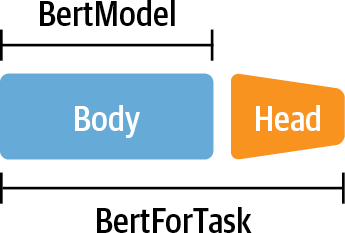
\includegraphics[width=0.2\textwidth]{images/bert-ner-body-head.png}
    \caption{BERT model body \& task-specific classification head (\cite{tunstall_natural_2022})}
    \label{fig:bert-ner-body-head}
\end{figure}

In simple terms, BERT converts sentences into vector representations (called embeddings) that machines can understand. Then the classification head uses this encoded "understanding" to give the words labels LOC, ORG and PER.


\section{Tokenization: Small Bites, Big Data}
Transformer models cannot receive raw strings as input. Instead, they assume the text has been tokenized and encoded as numerical vectors. (\cite{tunstall_natural_2022})

%Before words can be turned into vectors,
Prior to being fed into the model, the sentence undergoes a pre-processing step called tokenization, during which it is broken down from a string into the atomic units used in the model. (\cite{tunstall_natural_2022})

BERT uses subword tokenization WordPiece, which means that words are first split into smaller, more frequently occurring subword units called tokens. The WordPiece tokenizer converts each token to a corresponding index in the model's vocabulary called an input ID. Each input ID represents a unique token in the vocabulary. (\cite{tunstall_natural_2022}) The final output of the tokenizer is a sequence of word IDs (as seen in Table \ref{tab:tokenizer output}). Consider the example in \ref{tab:tokenizer output}:

\begin{table}[ht]
  \centering
  \begin{tabular}{c|c|c}
    %\hline
    \textbf{Raw Input} & \textbf{Tokens} & \textbf{Input IDs} \\
    \hline{}
    &  {\fontfamily{qcr}\selectfont [CLS]}  &  {\fontfamily{qcr}\selectfont 101}  \\ 
    My &  {\fontfamily{qcr}\selectfont My}  &  {\fontfamily{qcr}\selectfont 11590}  \\ 
    name &  {\fontfamily{qcr}\selectfont name}  &  {\fontfamily{qcr}\selectfont 11324}  \\ 
    is &  {\fontfamily{qcr}\selectfont is}  &  {\fontfamily{qcr}\selectfont 10124}  \\ 
    Elizaveta &  {\fontfamily{qcr}\selectfont Eliza}  &  {\fontfamily{qcr}\selectfont 59875}  \\ 
    &  {\fontfamily{qcr}\selectfont \#\#veta}  &  {\fontfamily{qcr}\selectfont 84379}  \\ 
    . &  {\fontfamily{qcr}\selectfont .}  &  {\fontfamily{qcr}\selectfont 119}  \\ 
    I'm &  {\fontfamily{qcr}\selectfont I}  &  {\fontfamily{qcr}\selectfont 146}  \\ 
    &  {\fontfamily{qcr}\selectfont '}  &  {\fontfamily{qcr}\selectfont 112}  \\ 
    &  {\fontfamily{qcr}\selectfont m}  &  {\fontfamily{qcr}\selectfont 181}  \\ 
    from &  {\fontfamily{qcr}\selectfont from}  &  {\fontfamily{qcr}\selectfont 10188}  \\ 
    Aberdeen &  {\fontfamily{qcr}\selectfont Aberdeen}  &  {\fontfamily{qcr}\selectfont 49317}  \\ 
    and &  {\fontfamily{qcr}\selectfont and}  &  {\fontfamily{qcr}\selectfont 10111}  \\ 
    I &  {\fontfamily{qcr}\selectfont I}  &  {\fontfamily{qcr}\selectfont 146}  \\ 
    study &  {\fontfamily{qcr}\selectfont study}  &  {\fontfamily{qcr}\selectfont 14687}  \\ 
    at &  {\fontfamily{qcr}\selectfont at}  &  {\fontfamily{qcr}\selectfont 10160}  \\ 
    the &  {\fontfamily{qcr}\selectfont the}  &  {\fontfamily{qcr}\selectfont 10105}  \\ 
    University &  {\fontfamily{qcr}\selectfont University}  &  {\fontfamily{qcr}\selectfont 10404}  \\ 
    of &  {\fontfamily{qcr}\selectfont of}  &  {\fontfamily{qcr}\selectfont 10108}  \\ 
    St &  {\fontfamily{qcr}\selectfont St}  &  {\fontfamily{qcr}\selectfont 10838}  \\ 
    Andrews &  {\fontfamily{qcr}\selectfont Andrews}  &  {\fontfamily{qcr}\selectfont 29583}  \\ 
    . &  {\fontfamily{qcr}\selectfont .}  &  {\fontfamily{qcr}\selectfont 119}  \\ 
    &  {\fontfamily{qcr}\selectfont [SEP]}  &  {\fontfamily{qcr}\selectfont 102}  \\ 
    %\hline
  \end{tabular}
  \caption{Tokenized example}
  \label{tab:tokenizer output}
\end{table}

Subword tokenization is used in the BERT NLP model to handle out-of-vocabulary (OOV)  words and reduce vocabulary size (\cite{tunstall_natural_2022}).
The word {\fontfamily{qcr}\selectfont Elizaveta} demonstrates this; the prefix {\fontfamily{qcr}\selectfont \#\#} in {\fontfamily{qcr}\selectfont \#\#veta} means the preceding word was not whitespace, and any token with this prefix should be merged with the previous token when converting the tokens back into a string. It helps BERT break down words into smaller pieces to capture their meaning better. Additionally, it benefits BERT to keep this word out of the vocabulary, which lowers the vocabulary dimension. (\cite{tunstall_natural_2022}) The {\fontfamily{qcr}\selectfont BERT Base Cased} Tokenizer has vocabulary size $d_\text{v} = 119547$.

\subsubsection{Special Tokens}

Note the special tokens added by the tokenizer in Table \ref{tab:tokenizer output} - {\fontfamily{qcr}\selectfont[CLS]} and {\fontfamily{qcr}\selectfont[SEP]}. In its tokenization process, BERT uses several special tokens; their roles are described in Table \ref{tab:special-tokens}.

\begin{table}[ht]
  \centering
  \begin{tabular}{|p{4cm}|p{4cm}|p{4cm}|}
    \hline
    \textbf{{\fontfamily{qcr}\selectfont[CLS]}} & \textbf{{\fontfamily{qcr}\selectfont[SEP]}} & \textbf{{\fontfamily{qcr}\selectfont[MASK]}} \\
    \hline{}
    classification token &  separator token & mask token \\
    \hline
    Added to the beginning of every input sequence. Represents the start of a classification task. &  Used to separate two input sequences in a sequence-pair classification task. Also used to separate multiple sentences in a single input sequence. & Used during pre-training to mask some of the input tokens randomly. The BERT model is then trained to predict the original token from the masked token, which helps it learn contextualized representations. \\
    \hline
  \end{tabular}
  \caption{BERT Special Tokens (\cite{tunstall_natural_2022})}
  \label{tab:special-tokens}
\end{table}




\section{BERT Model Body}

The model body of BERT has four main components, illustrated in Figure \ref{fig:bert-model-body-overview}.

\begin{figure}[H]
    \centering
    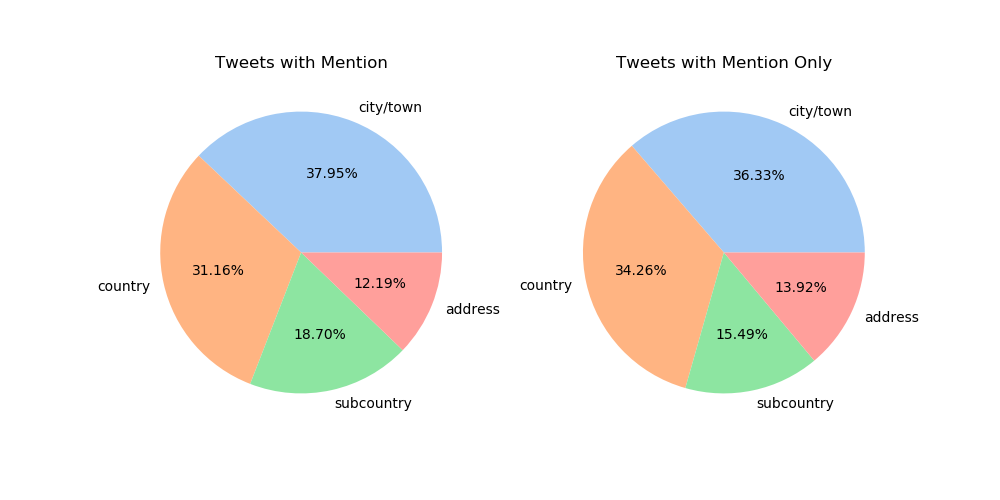
\includegraphics[width=0.5\textwidth]{images/mention_pie.png}
    \caption{BERT Model Body Structure}
    \label{fig:bert-model-body-overview}
\end{figure}

\begin{description}
   \item[Input Embeddings:] Input IDs obtained from the tokenization step are mapped to input embeddings using a lookup table (\cite{rohrer_transformers_2021}). These embeddings as starting points that are later adjusted to include more context (\cite{geron_hands-machine_2019}).
   
   \item[Positional Encoding:] The input embeddings do not contain information about where words are located in the input sentence. Positional encoding is added to the input sequence to fix this. (\cite{devlin_bert_2019})
   
   \item[Segment Embeddings:] \textcolor{red}{insert explanation}
   
   \item[Transformer Layers:] The token embeddings are then processed through multiple transformer layers, which use self-attention to capture the contextual relationships between tokens in the sequence. The transformer layers enable BERT to generate context-sensitive embeddings that capture the meaning of words based on their surrounding context. (\cite{devlin_bert_2019}) 
\end{description}

The output of the model body is an embedding vector for each token that captures its meaning in the context of the input sequence. \cite{tunstall_natural_2022}

Each of the above components is discussed in the subsequent sections.

Table \ref{tab:hyperparameters} shows the hyperparameters of BERT. 

\textcolor{red}{put hyperparameters in context and the table below as a summary}

\begin{table}[h]
\centering
\begin{tabular}{r|l}
\hline
    %\multicolumn{3}{c}{\textbf{Geotagged}} & \multicolumn{3}{c}{\textbf{Geotagged Only}} \\
    %\hline
    Hyper-parameter & Value \\
    \hline
     $d_\text{model}$ & $768$ \\
     $L$ & $12$ \\
     $A$ & $12$ \\
     $H$ & $768$ \\
     $d_\text{v}, d_\text{k}$ & $\frac{d_\text{model}}{A} = 64$ \\
     $d_{ff}$ & $4d_\text{model} = 3072$ \\
     \hline
\end{tabular}
\caption{BERT Base Body Hyperparameters \cite{devlin_bert_2019}}
\label{tab:hyperparameters}
\end{table}

%Now, onto discussing these components in proper, rigorous mathematical detail.


\section{All Great Models Begin With Input Embeddings}
The input embedding layer in BERT is a lookup table that maps each token in the input sequence to a high-dimensional vector representation (called the dimension of the model $d_\text{model} = 768$). The goal of the embedding layer is to transform the discrete input tokens into a continuous vector space where semantically similar words are closer to each other in this space. (\cite{rohrer_transformers_2021})

At this point, the word \textit{duck} has the same vector representation in both \textit{I saw her duck, it was so cute!} and \textit{I saw her duck down to hide}. The embeddings are not contextualised yet. Each token has an initial embedding that will later be adjusted to contain more information. (\cite{geron_hands-machine_2019})

In BERT, token IDs are often converted to one-hot vectors as an intermediate step in the process of obtaining token embeddings (\cite{tunstall_natural_2022}), (\cite{rohrer_transformers_2021}). Assume $ s = \begin{pmatrix} s_1 , s_2 , \dots , s_n \end{pmatrix} $ is a sequence of token IDs. Each token ID $s_j$ can be represented as a one-hot vector $S_j$, where $i = 1, \dots, d_{\text{vocab}}$:

$$ (S_j)_i = \begin{cases} 1 & \text{if } i = s_j \\ 0 & \text{otherwise} \end{cases} $$

Which can also be represented as a matrix of one-hot vectors $S \in \mathbb{R}^{n \times d_{\text{vocab}}}$.

$S$ is then multiplied by the lookup matrix $ L \in \mathbb{R}^{d_{\text{vocab}} \times d_{\text{model}}}$ to obtain the corresponding token embedding matrix $E \in \mathbb{R}^{n \times d_{\text{model}}}$.
$L$ contains the token embeddings for each token in the vocabulary. (\cite{geron_hands-machine_2019})

Consider the first row of $S$, which corresponds to $s_1$ token ID. If $1$ is in 101th place, only the 101th row of $L$ will be extracted. The first row of matrix $E$ will then correspond to the input embedding associated with 101th token.

$$
\underbrace{
    \begin{pmatrix}
    0 & \cdots & 0 & 1 & 0 & \cdots & 0 \\
    0 & \cdots & 0 & 0 & 0 & \cdots & 0 \\
    \vdots & \ddots & \vdots & \vdots & \vdots & \ddots & \vdots \\
    0 & \cdots & 0 & 0 & 0 & \cdots & 0
    \end{pmatrix}
}_{S\in \mathbb{R}^{n \times d_{\text{v}}}}
\overbrace{
    \begin{pmatrix}
    \cdots & \cdots & \cdots & \cdots \\
    \cdots & \cdots & \cdots & \cdots \\
    0.273  & 0.128  & \cdots & 0.879 \\
    \cdots & \cdots & \cdots & \cdots \\
    \cdots & \cdots & \cdots & \cdots \\
    \cdots & \cdots & \cdots & \cdots \\
    \cdots & \cdots & \cdots & \cdots \\
    \cdots & \cdots & \cdots & \cdots
    \end{pmatrix}
}^{L \in \mathbb{R}^{d_{\text{vocab}} \times d_{\text{model}}}}
=
\underbrace{
    \begin{pmatrix}
    0.273 & 0.128 & \cdots & 0.879 \\
    \cdots & \cdots & \cdots & \cdots \\
    \cdots & \cdots & \cdots & \cdots \\
    \cdots & \cdots & \cdots & \cdots
    \end{pmatrix}
}_{E \in \mathbb{R}^{n \times d_{\text{model}}}}
$$

$E$ has $n$ rows with each row $j$ representing the embedding of the $j$-th token.



\section{Positional Encoding}
Language models process text, which is sequential data. The positions of words in a sentence do not have any inherent meaning but are still crucial to the meaning of the sentence. Therefore, positional encoding is used to enable BERT to process the sequence of words in a sentence.

The positional encoding matrix $E \in \mathbb{R}^{n} \times d_{\text{model}}$ is defined as follows (\cite{geron_hands-machine_2019}):

$$ \text{P}_{i,j} =
\begin{cases}
\sin\left(\frac{i}{10000^\frac{j}{d_{\text{model}}}}\right)
& \text{if } j \text{ even} \\
\cos\left(\frac{i}{10000^\frac{j-1}{d_{\text{model}}}}\right)
& \text{if } j \text{ odd}
\end{cases} $$

where $\text{P}_{(i,j)}$ is the positional encoding for the $i$-th token and $j$-th dimension in the embedding vector, $d_{\text{model}}$ is the size of the embedding vector, and $i = 1, \dots, n$ and $j = 1, \dots, d_{\text{model}}$. The sine and cosine functions alternate for each position in the vector. The exponents $\frac{j}{d_{\text{model}}}$ and $\frac{j-1}{d_{\text{model}}}$ ensure that the encoding values have a unique pattern for each position in the sequence. (\cite{geron_hands-machine_2019})

The maximum sequence length BERT can handle is set to $n = 512$ (\cite{devlin_bert_2019}), so the positional encoding values are pre-computed and stored for all possible positions in a sequence of length 512.
The appropriate positional encoding values are selected and added to the corresponding token embeddings for the input sequence during training and inference. (\cite{geron_hands-machine_2019})

Using sine and cosine functions in the positional encoding ensures that the model can distinguish between tokens based on their relative position in the sequence. (\cite{geron_hands-machine_2019})

$\sin$ and $\cos$ functions are used because they are periodic (allowing them to capture relative positions of words regardless of sentence length), orthogonal (allowing them to represent different aspects of positional information without interfering with each other) and differentiable (necessary for training deep learning models like BERT). \cite{vaswani_attention_2017} (the team behind the original transformers) found that learned positional embeddings and sinusoidal positional encodings produced nearly identical results. 



\section{Segment Embeddings}
$$ \text{S}_{i} =
\begin{cases}
\sin\left(\frac{i}{10000^\frac{j}{d_{\text{model}}}}\right)
& \text{if } j \text{ even} \\
\cos\left(\frac{i}{10000^\frac{j-1}{d_{\text{model}}}}\right)
& \text{if } j \text{ odd}
\end{cases} $$

The positional encoding is added to the token embeddings before being fed into the transformer layers, allowing the model to use the sequential information to capture the context and meaning of the tokens in the input sequence. 
To get the final input embeddings for our sentence, the embedding matrix $E$ is added to the positional embedding matrix $P$. 
$$E + P = \textbf{x} \in  \mathbb{R}^{n \times d_{\text{model}}}$$
Since each row in $E$ corresponds to an input embedding of a token, adding $P$ is essentially adding the token location information to the input embedding.

\textcolor{red}{segment embeddings}
https://aclanthology.org/2022.lrec-1.152.pdf

\section{Power in numbers: Transformer Blocks}

The input sequence of embeddings
$\mathbf{x} \in \mathbb{R}^{n \times d_{\text{model}}}$ is passed into the first encoder block all at once, and the output of that block is then passed through the next transformer block until the sequence has been passed through all $L = 12$ blocks. The final output of the encoder is the encoded representation of $\mathbf{x}$. (\cite{thickstun_transformer_2020})

An encoder block can therefore be thought of as a function $f: \mathbb{R}^{n \times d_{\text{model}}} \rightarrow \mathbb{R}^{n \times d_{\text{model}}}$
where $f(\mathbf{x}) = \mathbf{z} \in \mathbb{R}^{n \times d_{\text{model}}}$, and the encoder can be thought of as composition $f_L \circ f_{L-1} \circ \dots \circ f_1$. (\cite{thickstun_transformer_2020})

This can also be illustrated by the diagram:

\begin{figure}[H]
    \centering
    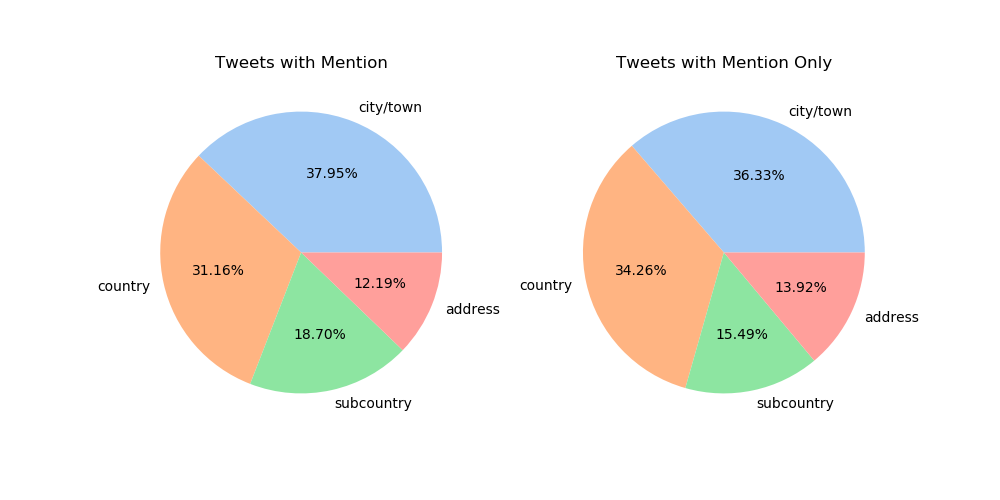
\includegraphics[width=0.5\textwidth]{images/mention_pie.png}
    \caption{Transformer Block}
    \label{fig:transformer-block}
\end{figure}

Each encoding transformer block consists of a stack of multiple identical transformer blocks, each of which consists of two sub-layers: a multi-head self-attention layer (MHA) and a position-wise feedforward network (FFN). \cite{vaswani_attention_2017}

The function $f$ can be written as:

$$f(\mathbf{x}) = \mathbf{z}$$
\begin{equation} \label{sublayer1}
    \mathbf{u}= \text{LayerNorm}(\mathbf{\mathbf{x}} + \text{MHA}(\mathbf{x}))
\end{equation}
\begin{equation} \label{sublayer2}
    \mathbf{z} = \text{LayerNorm}(\mathbf{u} + \text{FFN}(\mathbf{\mathbf{u}}))
\end{equation}

\subsection{Multi-Head Attention}

\subsubsection{What is attention?}
The attention mechanism enables neural networks to assign varying degrees of importance or attention to individual elements within a sequence. "Self" in self-attention refers to the fact that the computation of attention weights is performed based on the hidden states of the same sequence rather than using external context or information from another sequence. 
Self-attention involves using the entire sequence to determine the weight of each token's embedding rather than assigning a fixed embedding to each token. In other words, self-attention generates a new sequence of embeddings ($y_1, \dots, y_n$) based on a given sequence of token embeddings ($x_1, \dots, x_n$). Each new embedding $y_i$ is a weighted sum of all the token embeddings $x_j$, where the attention weights $w_{ij}$ are normalized such that $\sum_{}^{} w_{i,j} = 1$. (\cite{tunstall_natural_2022})
$$y_i = \sum_{j=1}^{n} w_{i,j} x_j$$
In the "duck" example, without context, the word might refer to a type of bird. However, with additional context, such as "I saw her duck to hide," it is clear that it pertains to the verb. To create a representation of "duck" that captures this context, all the token embeddings can be blended in various proportions by assigning greater weights $w_{ij}$ to the embeddings for "to" and "hide." These embeddings produced through this process are referred to as contextualized embeddings.

In BERT's multi-head attention layer, the attention mechanism is called "scaled dot-product attention" and is applied $A = 12$ times to the input sequence in parallel. (\cite{tunstall_natural_2022})


\subsubsection{Scaled Dot-Product Attention}

The input
$\mathbf{x} \in \mathbb{R}^
{n \times d_{\text{model}}}$
is first multiplied by projection matrices
$\mathbf{W}^Q, \mathbf{W}^K \in \mathbb{R}^
{d_{\text{model}} \times d_{\text{k}}}$
,
$\mathbf{W}^V \in \mathbb{R}^
{d_{\text{model}} \times d_{\text{v}}}$
to get the query, key and value matrices:
$ \mathbf{W}^Q \mathbf{x} = \mathbf{Q} \in \mathbb{R}^
{n \times d_{\text{k}}}$, 
$ \mathbf{W}^K  \mathbf{x} = \mathbf{K} \in \mathbb{R}^
{n \times d_{\text{k}}}$, 
$ \mathbf{W}^V \mathbf{x} = \mathbf{V} \in \mathbb{R}^
{n \times d_{\text{v}}}$. (\cite{thickstun_transformer_2020})
Note that each row in $\mathbf{x}$ is an embedding for each of the $n$ tokens in the sequence. By multiplying by $\mathbf{W}^Q, \mathbf{W}^K, \mathbf{W}^V$, each embedding vector is projected into three vectors (known as query, key and value) (\cite{tunstall_natural_2022}).

The attention scores are calculated using a similarity function, which is the "dot product." This is done by multiplying matrices $\mathbf{Q}\mathbf{K}^T \in \mathbb{R}^
{n \times n}$, which corresponds to attention scores for each token $n$. (\cite{tunstall_natural_2022})

The attention scores are multiplied by a scaling factor $d_{\text{k}}$ to smooth gradients during training by normalizing their variance (\cite{geron_hands-machine_2019}). Then the result is passed through the softmax function \cite{geron_hands-machine_2019}, so all column values sum to 1 to get the attention weights:
$$\text{softmax}(\frac{\mathbf{Q}\mathbf{K}^T}{\sqrt{d_k}}) \in  \mathbb{R}^
{n \times n}$$

For a given input matrix $X$ of shape $(m, n)$, where m is the number of rows and n is the number of columns, the softmax function \cite{geron_hands-machine_2019} is defined as:

$$ \mathrm{softmax}(X_{i,j}) = \frac{e^{X_{i,j}}}{\sum_{k=1}^m e^{X_{k,j}}} $$

where $i$ is the row index and $j$ is the column index.


\begin{figure}[H]
    \centering
    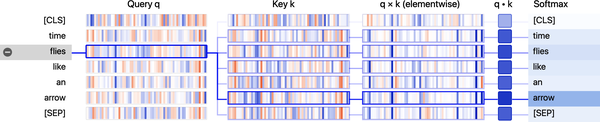
\includegraphics[width=1\textwidth]{images/QKV.png}
    \caption{Visualisation of Attention Mechanism}
    \label{fig:attention}
\end{figure}

The attention weights are multiplied by the values matrix to complete the scaled dot-product attention step (\cite{tunstall_natural_2022}). This results in an updated representation of each embedding:

\begin{align*}
    Attention(\mathbf{Q}, \mathbf{K}, \mathbf{V}) = softmax(\frac{\mathbf{Q}\mathbf{K}^T}{\sqrt{d_k}})\mathbf{V}
\end{align*}

This step can be summarised in terms of equations by:

$$ \mathbf{Q} = \mathbf{W}^Q \mathbf{x} \in \mathbb{R}^
{n \times d_{\text{k}}}$$
$$ \mathbf{K} = \mathbf{W}^K  \mathbf{x} \in \mathbb{R}^
{n \times d_{\text{k}}}$$
$$ \mathbf{V} = \mathbf{W}^V \mathbf{x} \in \mathbb{R}^
{n \times d_{\text{v}}}$$

\begin{align*}
    \text{head} = Attention(\mathbf{Q}, \mathbf{K}, \mathbf{V}) = softmax(\frac{\mathbf{Q}\mathbf{K}^T}{\sqrt{d_k}})\mathbf{V}
\end{align*}

\subsubsection{Multi-Head Attention}

Multi-head attention is a variant of scaled dot-product attention that splits the input into multiple "heads" and computes the attention for each head separately (\cite{tunstall_natural_2022}). So for each head $ a = 1, \dots, A$:

\begin{align*}
    \text{head}_a = Attention(\mathbf{Q}_a, \mathbf{K}_a, \mathbf{V}_a) = softmax(\frac{\mathbf{Q}_{a}\mathbf{K}_{a}^T}{\sqrt{d_k}})\mathbf{V}_a
\end{align*}

where 
$$ \mathbf{Q}_a = \mathbf{W}_a^Q \mathbf{x} \in \mathbb{R}^
{n \times d_{\text{k}}}$$
$$ \mathbf{K}_a = \mathbf{W}_a^K \mathbf{x} \in \mathbb{R}^
{n \times d_{\text{k}}}$$
$$ \mathbf{V}_a = \mathbf{W}_a^\mathbf{V} \mathbf{x} \in \mathbb{R}^
{n \times d_{\text{v}}}$$

Then outputs of $\text{head}_a$ are concatenated and projected using $\mathbf{W}^O \in \mathbb{R}^
{Ad_v \times d_{\text{model}}}$ (\cite{vaswani_attention_2017}).

\begin{align*}
    MHA(\mathbf{Q}, \mathbf{K}, \mathbf{V}) = \text{Concat}(\text{head}_1, \dots, \text{head}_A)\mathbf{W}^O
\end{align*}

Remember, by definition $d_v = d_\text{model}/A = 64$, so  $\mathbf{u} = MHA(\mathbf{Q}, \mathbf{K}, \mathbf{V}) \in \mathbb{R}^
{n \times d_{\text{model}}}$.

Note that the projection matrices $\mathbf{W}_a^Q$, $\mathbf{W}_a^K$, $\mathbf{W}_a^V$, $\mathbf{W}^O$ are learnable projection matrices. For now, assume they work. How they are learned is discussed in Section %\ref{gradient-descent}.

\subsection{Layer Normalisation 1}

Remember that the output of the first sublayer of the encoder block (\ref{sublayer1}) contains a residual connection, i.e., the original output $\mathbf{x}$ is added to the output of the MHA layer. The resulting sum is then passed through a layer normalization step. This "Add \& Norm" layer can be mathematically represented (\cite{thickstun_transformer_2020}) as:

$$\text{AddNorm}(\mathbf{x}) = \text{LayerNorm}(\mathbf{x} + \text{MHA}(\mathbf{x}); \alpha_1, \beta_1)$$

For a given input matrix $ X \in \mathbb{R}^
{n \times m}$, the layer normalization function is defined as:

\begin{equation} \label{layernorm}
    \mathrm{LayerNorm}(X_{i}) = \alpha_1\frac{X_{i} - \mu_i}{\sqrt{\sigma_i^2 + \epsilon}} + \beta_1 
\end{equation}

$$\mu_i = \frac{1}{n}\sum_{j=1}^n X_{i,j}$$

$$\sigma_i = \sqrt{\frac{1}{n}\sum_{j=1}^n (X_{i,j}-\mu_i)^2}$$

where $i$ is the row index, $\mu_i$ is the mean of the $i$-th row, $\sigma_i$ is the standard deviation of the $i$-th row (\cite{thickstun_transformer_2020}), and $\epsilon$ is a small constant added to avoid division by zero (\cite{huang_annotated_2022}), $\alpha_1, \beta_1 \in \mathbb{R}^{n}$ are learned parameters (\cite{thickstun_transformer_2020}).

Residual connections and layer normalization help alleviate the vanishing gradient problem and improve the stability of the training process. (\cite{vaswani_attention_2017})

\subsection{Feed-Forward Network}

Moving onto the second sublayer (\ref{sublayer2}).
The position-wise feedforward network consists of two linear transformations with a ReLU activation function in between, which enables the model to capture complex non-linear relationships between the input sequence and the output embeddings.

The feedforward sublayer of the Transformer block takes the output of the MHA sublayer and applies a two-layer fully connected neural network to each token in the input sequence. The feedforward sublayer can be mathematically represented (\cite{vaswani_attention_2017}) as follows:

\begin{equation}
    \text{FFN}(\mathbf{x}) = \text{ReLU}(\mathbf{x} \mathbf{W}_1 + \mathbf{b}_1) \mathbf{W}_2 + \mathbf{b}_2 
     = \max(0, \mathbf{x} \mathbf{W}_1 + \mathbf{b}_1) \mathbf{W}_2 + \mathbf{b}_2
\end{equation}

where $\mathbf{x}$ is the output of the self-attention sublayer, $\mathbf{W}_1 \in \mathbb{R}^
{d_{\text{model}} \times d_{ff}}$ and $\mathbf{W}_2 \in \mathbb{R}^{d_{ff} \times d_{\text{model}}}$ are learnable weight matrices for the first and second layers of the fully connected network, respectively, and $\mathbf{b}_1 \in \mathbb{R}^{d_{ff}}$ and $\mathbf{b}_2 \in \mathbb{R}^{d_{\text{model}}}$ are learnable bias vectors for the first and second layers, respectively. $d_{ff}$ is the inner layer dimensionality, and in BERT $d_{ff} = 4d_\text{model} = 3072$.

\subsection{Layer Normalisation 2}

The output of the feedforward sublayer is then passed through another "Add \& Norm" sublayer, which can be mathematically represented as \cite{thickstun_transformer_2020}:

$$\text{AddNorm}(\mathbf{u}) = \text{LayerNorm}(\mathbf{u} + \text{FFN}(\mathbf{u}); \alpha_2, \beta_2)$$

\subsection{Summary of Transformer Block}

BERT has $L = 12$ encoder blocks, each of which can be defined as a function $f_l(\mathbf{x}) = z \in \mathbb{R}^{n \times d_{\text{model}}}$ where:
$$f_l(\mathbf{x}) = \mathbf{z}$$
\begin{equation}
    \mathbf{u}= \text{LayerNorm}(\mathbf{\mathbf{x}} + \text{MHA}(\mathbf{x}); \alpha_1, \beta_1)
\end{equation}
\begin{equation} 
    \mathbf{z} = \text{LayerNorm}(\mathbf{u} + \text{FFN}(\mathbf{\mathbf{u}}); \alpha_2, \beta_2)
\end{equation}
where MHA is defined as:
\begin{align*}
    \text{MHA}(\mathbf{Q}, \mathbf{K}, \mathbf{V}) = \text{Concat}(head_1, \dots, head_A)\mathbf{W}^O
\end{align*}
\begin{align*}
    \text{head}_a = \text{Attention}(\mathbf{Q}_a, \mathbf{K}_a, \mathbf{V}_a) = \text{softmax}(\frac{\mathbf{Q}_{a}\mathbf{K}_{a}^T}{\sqrt{d_k}})\mathbf{V}_a
\end{align*}
$$ \mathbf{Q}_a = \mathbf{W}_a^Q  \mathbf{x} \in \mathbb{R}^
{n \times d_{\text{k}}}$$
$$ \mathbf{K}_a = \mathbf{W}_a^K \mathbf{x} \in \mathbb{R}^
{n \times d_{\text{k}}}$$
$$ \mathbf{V}_a = \mathbf{W}_a^\mathbf{V}  \mathbf{x} \in \mathbb{R}^
{n \times d_{\text{v}}}$$

and FFN is defined as: 
$$\text{FFN}(\mathbf{x}) = \max(0, \mathbf{x} \mathbf{\mathbf{W}}_1 + \mathbf{b}_1) \mathbf{W}_2 + \mathbf{b}_2$$
The learnable parameters of the encoder block are shown in Table \ref{tab:bert-parameters}.

\begingroup
\setlength{\tabcolsep}{10pt} % Default value: 6pt
\renewcommand{\arraystretch}{1.5} % Default value: 1
\begin{table}[H]
\centering
    \begin{tabular}{c|c|c}
    \textbf{Layer} & \textbf{Parameters} & \textbf{Dimensions} \\ \hline
     MHA & $\mathbf{W}_a^Q, \mathbf{W}_a^K$ & $\mathbb{R}^{d_{\text{model}} \times d_{\text{k}}}$ \\
    
    & $\mathbf{W}_a^V$ & $\mathbb{R}^{d_{\text{model}} \times d_{\text{v}}}$ \\
    
    & $\mathbf{W}^O$ & $\mathbb{R}^{Ad_v \times d_{\text{model}}}$ \\ \hline
     
     FFN & $\mathbf{W}_1$ & $\mathbb{R}^{d_{\text{model}} \times d_{ff}}$ \\
     & $\mathbf{W}_2$ & $\mathbb{R}^{d_{ff} \times d_{\text{model}}}$ \\
     & $\mathbf{b}_1$ & $\mathbb{R}^{d_{ff}}$ \\
     & $\mathbf{b}_2$ & $\mathbb{R}^{d_{\text{model}}}$ \\ \hline
     
    LayerNorm & $\alpha_1, \beta_1$ & $\mathbb{R}^n$ \\
     & $\alpha_2, \beta_2$ & $\mathbb{R}^n$ \\ 
    \end{tabular}
\caption{Learnable Parameters of Encoder Block}
\label{tab:bert-parameters}
\end{table}
\endgroup





\section{Pre-Training}
Pre-training refers to the training of the body of the model.
In BERT, pre-training to learn the contextual representation of words is done through two tasks: Masked Language Modelling (MLM) and Next Sentence Prediction (NSP) (\cite{devlin_bert_2019}).

\subsection{Masked Language Modelling}

In Masked Language Modelling, a certain percentage of tokens are masked, and the training objective is to predict those masked tokens. In BERT, 15\% of tokens are masked during pre-training, meaning if the $i$-th token is masked, it is replaced with the {\fontfamily{qcr}\selectfont [MASK]} token 80\% of the time, the unchanged token 10\% of the time and a random token 10\% of the time (so there is no mismatch between pre-training and fine-tuning). Then {\fontfamily{qcr}\selectfont [MASK]} (the $i$-th token) is used to predict the original token with cross-entropy loss (type of loss function used in classification tasks). (\cite{devlin_bert_2019})

For example, in the sentence "I saw her {\fontfamily{qcr}\selectfont [MASK]} to hide.", the model has to predict the masked word "duck" based on the context of the rest of the sentence. BERT is forced to learn contextualized representations of all the words in the sequence because it does not know which word is masked. Remember that BERT takes into account both left and right contexts when making predictions.

The goal of pre-training is to train a model that can predict the masked words based on the context of the surrounding words. This is done by minimizing the cross-entropy loss between the predicted probabilities of the masked words and their true values. (\cite{devlin_bert_2019})

This is implemented by adding a classification layer on top of the encoder, multiplying the output vectors by the embedding matrix (so they are the dimension of the vocabulary) and calculating the probability of each word in the vocabulary with softmax. (\cite{devlin_bert_2019})

\subsection{Next Sentence Prediction}

In order to train a model that understands sentence relationships, BERT was pre-trained for a next sentence prediction task that involves predicting whether two sentences follow each other. Specifically, this is done by concatenating two sentences from the corpus to create inputs. During training, when choosing the sentences for each pre-training example, 50\% of the time the second sentence is the actual next sentence that follows the first sentence (labeled as {\fontfamily{qcr}\selectfont IsNext}), and 50\% of the time it is a random sentence from the corpus (labeled as {\fontfamily{qcr}\selectfont NotNext}) (\cite{devlin_bert_2019}).

To predict if the second sentence is indeed connected to the first, the following steps are performed:

The entire input sequence goes through the Transformer model. The output of the {\fontfamily{qcr}\selectfont [CLS]} token is fed into a simple classification layer. %(learned matrices of weights and biases).
The probability of {\fontfamily{qcr}\selectfont IsNextSequence} is calculated using softmax. (\cite{devlin_bert_2019})

When training the BERT model, MLM and NSP are trained together, with the goal of minimizing the combined loss function of the two strategies. (\cite{devlin_bert_2019})

Together, MLM and NSP enable BERT to learn contextualized representations of words, which can then be fine-tuned for a wide range of downstream NLP tasks.(\cite{devlin_bert_2019})


\section{Fine-Tuning}
Fine-tuning BERT refers to training the task-specific classification head. Fine-tuning BERT for NER involves adapting the pre-trained model to the specific task of identifying entities in text. Here are the general steps for fine-tuning BERT for NER:

\begin{description}
   \item[Data Preparation:] Prepare the NER data by labeling the entities in the text and splitting the data into training, validation, and test sets. There were several datasets used to train our model (due to it being multilingual). The labeled Spanish dataset (www.clips.uantwerpen.be, 2005) consists of two columns separated by a space, with each word (and punctuation symbol) on a new line next to its named entity tag, with a blank line between sentences (See Table \ref{tab:ner-dataset}, where B denotes the first item of the phrase and I denotes a non-initial word ).
\end{description}

\begin{table}[h]
\centering
    \begin{tabular}{ll}
    \hline
    \textbf{Text} & \textbf{Label} \\ \hline
    Wolff & B-PER \\
    , & O \\
    currently & O \\
    a & O \\
    journalist & O \\
    in & O \\
    Argentina & B-LOC \\
    , & O \\
    played & O \\
    with & O \\
    Del & B-PER \\
    Bosque & I-PER \\
    in & O \\
    the & O \\
    final & O \\
    years & O \\
    of & O \\
    the & O \\
    seventies & O \\
    in & O \\
    Real & B-ORG \\
    Madrid & I-ORG \\
    . & O \\ \hline
    \end{tabular}
\caption{Sample Sentence from BERT NER Training Dataset \cite{noauthor_language-independent_2005}}
\label{tab:ner-dataset}
\end{table}

\begin{description}
   \item[Tokenization \& Input Embeddings] Tokenize the input text using the BERT tokenizer and create token and segment ID embeddings for the input sequences. During the training process, the pre-trained body and the classification head parameters are fine-tuned using backpropagation and gradient descent optimization. \cite{merchant_what_2020}
   
   \item[Model Architecture:] Add a classification layer on top of the pre-trained BERT model that can identify the named entities in the input text. It typically consists of a fully connected layer and a softmax activation function. (\cite{tunstall_natural_2022})
   
   \item[Fine-tuning:] Fine-tune the pre-trained BERT model on the NER task using the training data. During fine-tuning, the pre-trained BERT model and classification head weights are updated based on the task-specific loss function. (\cite{devlin_bert_2019})
   
   \item[Validation \& Evaluation:] Validate the fine-tuned model on the validation set. Evaluate the fine-tuned model on the test set and report the performance metrics.
   
\end{description}

In summary, to fine-tune BERT for NER, the pre-trained BERT model is used as the base, a classification layer is added on top, and then fine-tune the model on the labeled NER data.


%\section{Gradient Descent} \label{gradient-descent}
%
Thus far it was taken for granted that the neural network could "learn". The weight matrices that are the crux to BERT's success materialised out of thin air to save the day. The reality is not quite so rosy. The reality invoves calculus.
In this section, the way in which BERT learns (particularly how the weight matrices are created) will be explained.

The way BERT learns is through backpropagation. 

\subsection{Gradient Descent in Terms of BERT}

Gradient descent is an optimization algorithm commonly used in machine learning to minimize a loss function. In the context of BERT, gradient descent is used to fine-tune the pre-trained base model and the classification head for a specific downstream task such as named entity recognition. 

Given a set of parameters $\theta$ and a loss function $J(\theta)$, the goal of gradient descent is to find the set of parameters that minimizes the loss function. Gradient descent does this by iteratively updating the parameters in the direction of the negative gradient of the loss function. The update rule is as follows:

$$\theta_{t+1} = \theta_t - \alpha \nabla J(\theta_t)$$

where $\theta_t$ represents the parameter values at iteration $t$, $\alpha$ is the learning rate, and $\nabla J(\theta_t)$ is the gradient of the loss function with respect to the parameters.

In the context of BERT, let's assume we have a set of training examples $(x_i, y_i)$, where $x_i$ is a sequence of tokens and $y_i$ is the corresponding set of named entity labels. We want to fine-tune the pre-trained BERT model to perform NER on this dataset. The loss function we want to minimize is the cross-entropy loss between the predicted named entity labels and the true labels:

$$J(\theta) = -\frac{1}{N} \sum_{i=1}^N \sum_{j=1}^M y_{ij} \log(\hat{y}{ij}) + (1 - y{ij}) \log(1 - \hat{y}_{ij})$$

where $\theta$ represents the parameters of the BERT model and the classification head, $N$ is the number of training examples, $M$ is the maximum sequence length, $y_{ij}$ is the true label for the $j$-th token in the $i$-th training example, and $\hat{y}{ij}$ is the predicted probability of the $j$-th token in the $i$-th training example being of the named entity type corresponding to $y{ij}$.

To update the parameters using gradient descent, we need to compute the gradient of the loss function with respect to the parameters. We can use backpropagation to compute this gradient efficiently. The update rule for gradient descent becomes:

$$\theta_{t+1} = \theta_t - \alpha \nabla J(\theta_t)$$

where $\nabla J(\theta_t)$ is the gradient of the loss function with respect to the parameters at iteration $t$.

In practice, the BERT-based NER model is trained using a variant of gradient descent called Adam, which uses adaptive learning rates and momentum to speed up convergence. However, the basic principles of gradient descent remain the same.



\subsection{Gradient Descent}

Gradient descent is an optimization algorithm used in machine learning to minimize the cost function of a neural network. It is used to update the weights and biases of the neural network by iteratively moving in the direction of steepest descent of the cost function. The gradient of the cost function with respect to the weights and biases is computed and used to update them in the opposite direction of the gradient.

The algorithm can be explained using the following steps:

Initialize the weights and biases of the neural network to random values.

Calculate the output of the neural network for a given input using the current weights and biases.

Compute the cost function for the output of the neural network. The cost function measures how well the network is performing on the given input.

Calculate the gradient of the cost function with respect to the weights and biases using backpropagation.

Update the weights and biases using the following equations:

\begin{align}
w_{ij} &:= w_{ij} - \alpha \frac{\partial J}{\partial w_{ij}} \
b_{j} &:= b_{j} - \alpha \frac{\partial J}{\partial b_{j}}
\end{align}

where $w_{ij}$ is the weight of the connection between neuron $i$ in the previous layer and neuron $j$ in the current layer, $b_{j}$ is the bias of neuron $j$ in the current layer, $\alpha$ is the learning rate (a hyperparameter that determines the step size of the update), and $\frac{\partial J}{\partial w_{ij}}$ and $\frac{\partial J}{\partial b_{j}}$ are the partial derivatives of the cost function with respect to the weights and biases, respectively.

Repeat steps 2-5 for all training examples in the dataset, for a fixed number of iterations (epochs) or until the cost function reaches a minimum.
The gradient descent algorithm can be further optimized using techniques such as batch gradient descent, stochastic gradient descent, and mini-batch gradient descent. Batch gradient descent computes the gradient of the cost function with respect to the weights and biases using the entire training dataset. Stochastic gradient descent computes the gradient for each training example individually. Mini-batch gradient descent computes the gradient for a small batch of training examples at a time.

In summary, gradient descent is an optimization algorithm used in machine learning to minimize the cost function of a neural network. It updates the weights and biases of the neural network by iteratively moving in the direction of steepest descent of the cost function, using the partial derivatives of the cost function with respect to the weights and biases. The learning rate controls the step size of the update, and different versions of gradient descent can be used depending on the size of the training dataset and the resources available.


\subsection{Backpropagation}

Backpropagation is a widely used algorithm for computing the gradient of the cost function with respect to the weights and biases of a neural network. The algorithm computes the gradient by recursively applying the chain rule of calculus to propagate the errors backwards from the output layer to the input layer.

The backpropagation algorithm can be explained using the following steps:

Forward propagation: Calculate the output of the neural network for a given input by passing it through the layers of the network, using the current weights and biases.

Compute the cost function for the output of the neural network. The cost function measures how well the network is performing on the given input.

Backward propagation: Compute the error of the output layer with respect to the cost function, and then recursively propagate this error backwards through the layers of the network.

The error of the output layer is given by:

\begin{equation}
\delta^{L}_j = \frac{\partial J}{\partial a^{L}_j} \sigma^{\prime}(z^{L}_j)
\end{equation}

where $J$ is the cost function, $a^{L}_j$ is the output of neuron $j$ in the output layer, $z^{L}_j$ is the weighted input of neuron $j$ in the output layer, $\sigma$ is the activation function, and $\sigma^{\prime}$ is its derivative. The partial derivative of the cost function with respect to the output of neuron $j$ in the output layer is given by:

\begin{equation}
\frac{\partial J}{\partial a^{L}_j}
\end{equation}

The error is then propagated backwards to the previous layer using the following equation:

\begin{equation}
\delta^{l}j = (\sum_k w{jk}\delta^{l+1}_k) \sigma^{\prime}(z^{l}_j)
\end{equation}

where $w_{jk}$ is the weight of the connection between neuron $j$ in layer $l$ and neuron $k$ in layer $l+1$, and $\delta^{l+1}_k$ is the error of neuron $k$ in layer $l+1$.

Compute the partial derivative of the cost function with respect to the weights and biases using the errors propagated backwards through the layers. The partial derivative of the cost function with respect to the weight $w_{ij}$ is given by:
\begin{equation}
\frac{\partial J}{\partial w_{ij}} = a^{l-1}_i \delta^{l}_j
\end{equation}

The partial derivative of the cost function with respect to the bias $b_j$ is given by:

\begin{equation}
\frac{\partial J}{\partial b_j} = \delta^{l}_j
\end{equation}

Use the computed partial derivatives to update the weights and biases using an optimization algorithm such as gradient descent.

In summary, backpropagation is an algorithm used to compute the gradient of the cost function with respect to the weights and biases of a neural network. The algorithm recursively propagates the errors backwards from the output layer to the input layer, and uses these errors to compute the partial derivatives of the cost function with respect to the weights and biases. These partial derivatives are then used to update the weights and biases using an optimization algorithm such as gradient descent.


 
\chapter{Results} %SB - URGENT
The aim of this paper is to evaluate for the purpose of determining travel patterns of Argentinian residents.
The exploratory data analysis aimed to describe the tweets based on whether they had a location mention, a geotag or both.

%The questions we aimed to answer with the exploratory data analysis
%\begin{enumerate}
%    \item What are the mentioned locations in tweets?
%    \item What are the geotagged locations in tweets?
%    \item How often are mentioned locations the same as geotagged locations?
%\end{enumerate}

Geotagged tweets were defined as those that contain a non-null Place and Coordinate objects. Mentioned tweets were defined as those that contained an NER tag {\fontfamily{qcr}\selectfont LOC} in the tweet content. Geoparsed tweets were mentioned tweets that have been mapped to coordinates by Google Geolocator API.

\section{Composition of the Tweet Collection}

There were a total of 182,571,272 tweets from 89,369 users whose tweets were collected and processed.
56435136 (30.91\%)  of those tweets were geotagged,  7,269,062 (3.98\%) had a location mention,  3,186,664 (1.75\%) had a geoparsed location. There were 3,015,837  tweets that had both a geotag and a location mention (corresponding to 82342  users); of which  1,722,811  tweets have a geotag and geoparsed location (corresponding to 72898  users). 

Over the relevant time period, Table \ref{fig:results-venn-diagram} shows the summary statistics of tweets per user.

Figure \ref{fig:results-venn-diagram} shows the overlap between geotagged, mentioned, and geoparsed tweets among the total collected tweets.
Users may have had more than one mentioned location per tweet, and had varying patterns of geotagging and mentioning.
A small subset of users were found to have very high rates of geotagging/mentioning and upon closer inspection, appeared to be event promoters or similar accounts.

\begin{figure}[H]
    \centering
    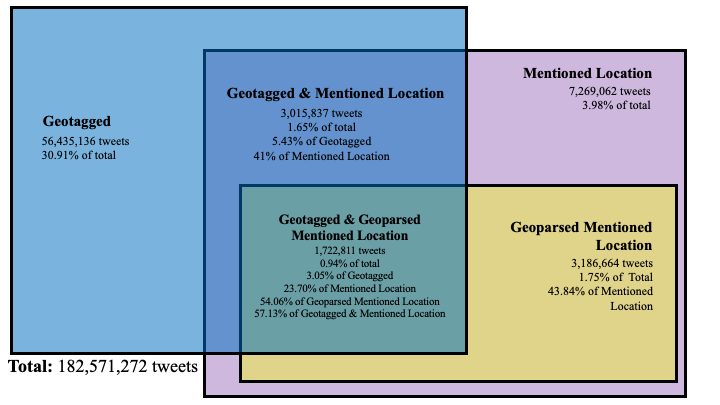
\includegraphics[width=1\textwidth]{images/Results-Venn-Diagram.png}
    
    \caption{Summary of Collected Tweets}
    \label{fig:results-venn-diagram}
\end{figure}

\begin{table}[htbp]
    \centering
    \begin{tabular}{|c|c|c|c|c|}
    \hline
    \textbf{Metric} & \textbf{Total} & \textbf{Geotagged} & \textbf{Mentioned} & \textbf{Geoparsed}\\
    \hline
    Mean &  2042.89  &  631.77  &  83.00  &  38.25 \\
    
    Median &  1164.0  &  286.0  &  34.0  &  13.0 \\
    
    Max &  155484  &  155464  &  79546  &  74832 \\
    
    Min &  1  &  1  &  1  &  1 \\ 
    
    Std &  2822.51  &  1208.67  &  397.92  &  329.78 \\
    \hline
    \end{tabular}
    \caption{Summary of Number of Tweets per User}
    \label{tab:summary-users}
\end{table}

%\begin{figure}[H]
%    \centering
%    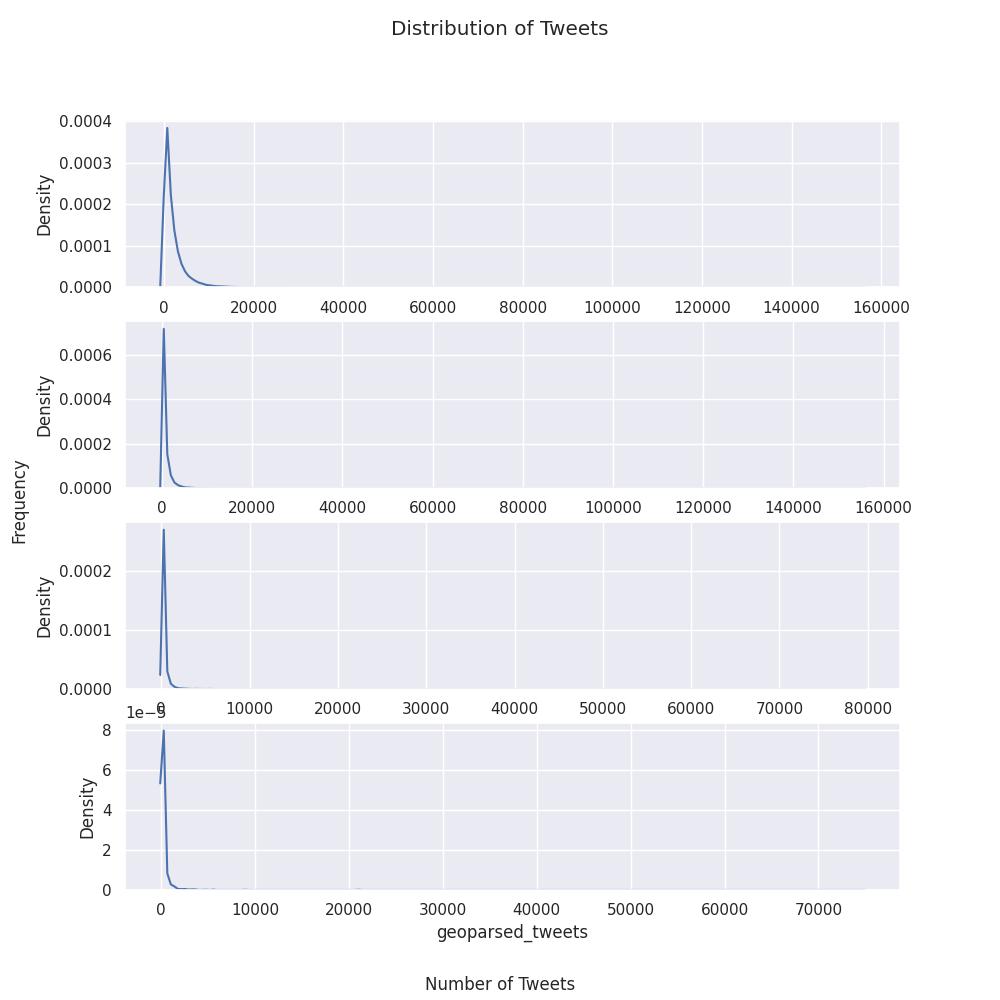
\includegraphics[width=1\textwidth]{images/user_tweets.png}
    
%    \caption{Number of Tweets per User - Total, Geotagged, Mentioned, Geoparsed}
%    \label{fig:user-tweets}
%\end{figure}

The number of users that tweeted only from Argentina was 188 (based on geotag), which is  0.21\% of the total users.

Different types of location information was available for each type of tweet. Mentioned tweets that have been geoparsed have address, city/town, subcountry, country-level granularity based on the output of Google Geolocator API. Geotagged tweets have two main fields for describing location: place name and country. It is difficult to determine how granular the mentioned location is as some place names are counties, while others are names of museums or night clubs, and others still are countries.

\pagebreak
\section{Geotagged}

Geotagged information is not divided into levels of granularity, though it would be possible to determine granularity if geotagged information were geoparsed like the mentioned locations.
Every geotagged tweet has a Place object with attributes name, full name, country and country code. The name is usually a town/city or country, but nothing I could determine that would indicate this granularity. Since the Place object has a country element, it is possible to determine country-level information for downstream analysis.

Geotagged tweets have {\fontfamily{qcr}\selectfont place\_name} and {\fontfamily{qcr}\selectfont place\_country} attributes. 

\subsection{All Countries}

By using the country-level information associated with geotagged tweets, the most geotagged countries were found. Table \ref{table:geotagged-countries}(a) shows the 20 countries with the most number of geotags.


For each user, the countries they geotagged over the course of the relevant time period were found. The 20 most popular geotagged countries are shown in Table \ref{table:geotagged-countries}(b).

\begin{table}
\centering
\begin{subtable}[c]{0.5\textwidth}
\centering
    \begin{tabular}{|c|c|c|}
    \hline
    Location & Number of Tweets & Proportion \\
    \hline
    Argentina & 55743738 & 0.987525 \\
    United States & 152911 & 0.002709 \\
    Brazil & 128727 & 0.002280 \\
    Chile & 68889 & 0.001220 \\
    Uruguay & 55464 & 0.000983 \\
    Spain & 36813 & 0.000652 \\
    Mexico & 30013 & 0.000532 \\
    Paraguay & 29848 & 0.000529 \\
    Colombia & 18635 & 0.000330 \\
    Italy & 15074 & 0.000267 \\
    United Kingdom & 14844 & 0.000263 \\
    Venezuela & 14505 & 0.000257 \\
    Ecuador & 13178 & 0.000233 \\
    France & 12456 & 0.000221 \\
    Russia & 9022 & 0.000160 \\
    Peru & 8327 & 0.000148 \\
    Germany & 6775 & 0.000120 \\
    Japan & 5729 & 0.000101 \\
    Dominican Republic & 5140 & 0.000091 \\
    Canada & 5104 & 0.000090 \\
    Other & 67692 & 0.001199 \\
    \hline
    \end{tabular}
\subcaption{in Tweets}
\end{subtable}

\begin{subtable}[c]{0.5\textwidth}
\centering
    \begin{tabular}{|c|c|c|}
    \hline
    Location & Number of Tweets & Proportion \\
    \hline
    Argentina & 89329 & 0.723072 \\
    Brazil & 6008 & 0.048632 \\
    United States & 5410 & 0.043791 \\
    Chile & 2970 & 0.024041 \\
    Uruguay & 2113 & 0.017104 \\
    Mexico & 1693 & 0.013704 \\
    Spain & 1681 & 0.013607 \\
    Italy & 1017 & 0.008232 \\
    Peru & 959 & 0.007763 \\
    United Kingdom & 939 & 0.007601 \\
    Paraguay & 938 & 0.007593 \\
    France & 883 & 0.007147 \\
    Colombia & 788 & 0.006378 \\
    Dominican Republic & 444 & 0.003594 \\
    Germany & 429 & 0.003473 \\
    The Netherlands & 402 & 0.003254 \\
    Ecuador & 393 & 0.003181 \\
    Japan & 280 & 0.002266 \\
    Venezuela & 267 & 0.002161 \\
    Panama & 266 & 0.002153 \\
    Other & 6332 & 0.051254 \\
    \hline
    \end{tabular}
\caption{by Users}
\end{subtable}
\caption{Most Commonly Geotagged Countries}
\label{table:geotagged-countries}
\end{table}

For the top 5 most geotagged countries in Table \ref{table:geotagged-countries} (excluding Argentina), the number of tweets and the number of users geotagging those countries was was found for each epi week (see Figure \ref{fig:geotagged-countries-tweets-epi-week} and Figure \ref{fig:geotagged-countries-users-epi-week}).

%\begin{figure}[H]
%        \centering
\begin{figure}[H]%{.49\linewidth}
    \centering
    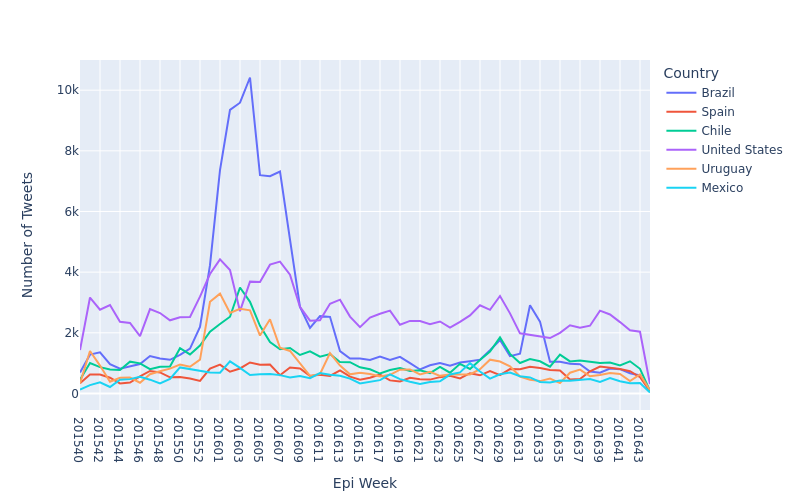
\includegraphics[width=1\textwidth]{images/geotagged_tweets_country_epi_week.png}
    \caption{by Tweets}
    \label{fig:geotagged-countries-tweets-epi-week}
\end{figure}
%        \hfill


\begin{figure}[H]%{.49\linewidth}
    \centering
    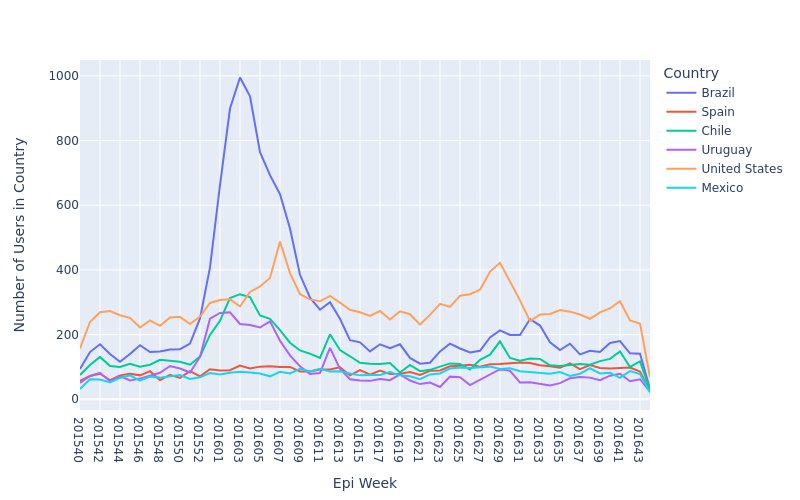
\includegraphics[width=1\textwidth]{images/geotagged_users_country_epi_week.png}
    \caption{by User}
    \label{fig:geotagged-countries-users-epi-week}
\end{figure}
%        \caption{Distribution of Most Geotagged Countries}
%        \label{fig:geotagged-countries-epi-week}
%\end{figure}

%Figure \ref{fig:mentioned-tweets-argentina-epi-week} shows the number of times Argentina was mentioned in tweets during each epi week.

\subsection{Argentina}

By considering {\fontfamily{qcr}\selectfont place\_name}, the the most commonly geotagged locations in tweets in Argentina were found (see Table \ref{table:mentioned-argentina}(a). Similarly, the most commonly geotagged locations by users in Argentina are shown in Table \ref{table:mentioned-argentina}(b).

\begin{table}
\centering
\begin{subtable}[c]{0.5\textwidth}
\centering
    \begin{tabular}{|c|c|c|}
    \hline
    Location & Number of Tweets & Proportion \\
    \hline
    Ciudad Autónoma de Buenos Aires & 6013615 & 0.107880 \\
    Córdoba & 4963649 & 0.089044 \\
    Buenos Aires & 3530325 & 0.063331 \\
    La Plata & 1824224 & 0.032725 \\
    Rosario & 1787751 & 0.032071 \\
    Santa Fe & 1258011 & 0.022568 \\
    Mar del Plata & 1136730 & 0.020392 \\
    Entre Ríos & 1108310 & 0.019882 \\
    Corrientes & 1076449 & 0.019311 \\
    Neuquén & 913416 & 0.016386 \\
    Lomas de Zamora & 806670 & 0.014471 \\
    Río Negro & 786264 & 0.014105 \\
    Bahía Blanca & 751970 & 0.013490 \\
    Santa Fé & 742449 & 0.013319 \\
    Lanús Oeste & 735798 & 0.013200 \\
    Almirante Brown & 700483 & 0.012566 \\
    Quilmes & 697071 & 0.012505 \\
    González Catán & 687619 & 0.012335 \\
    Mendoza & 657052 & 0.011787 \\
    Ciudad del Libertador General San Martín & 602969 & 0.010817 \\
    Other & 24361219 & 0.437022 \\
    \hline
    \end{tabular}
\subcaption{in Tweets}
\end{subtable}
\begin{subtable}[c]{0.5\textwidth}
\centering
    \begin{tabular}{|c|c|c|}
    \hline
    Location & Number of Tweets & Proportion \\
    \hline
    Ciudad Autónoma de Buenos Aires & 40660 & 0.093223 \\
    Buenos Aires & 31355 & 0.071889 \\
    Córdoba & 18180 & 0.041682 \\
    Villa Soldati & 9549 & 0.021893 \\
    Santa Fe & 9251 & 0.021210 \\
    La Plata & 9196 & 0.021084 \\
    Rosario & 8842 & 0.020272 \\
    Mar del Plata & 7868 & 0.018039 \\
    Entre Ríos & 7867 & 0.018037 \\
    San Isidro & 7216 & 0.016544 \\
    Tigre & 7098 & 0.016274 \\
    Avellaneda & 6644 & 0.015233 \\
    Vicente López & 6390 & 0.014651 \\
    González Catán & 6357 & 0.014575 \\
    Argentina & 6252 & 0.014334 \\
    Ciudad del Libertador General San Martín & 6132 & 0.014059 \\
    Morón & 5888 & 0.013500 \\
    Lomas de Zamora & 5577 & 0.012787 \\
    Caseros & 5244 & 0.012023 \\
    Buenos Aires City Region & 4966 & 0.011386 \\
    Other & 225628 & 0.517306 \\
    \hline
    \end{tabular}
\caption{by Users}
\end{subtable}
\caption{Most Commonly Geotagged Locations in Argentina}
\label{table:geotagged-argentina}
\end{table}

The distribution of tweets geotagged with Argentina over the course of the relevant time period is shown in Figure \ref{fig:geotagged-tweets-argentina-epi-week}

\begin{figure}[H]
    \centering
    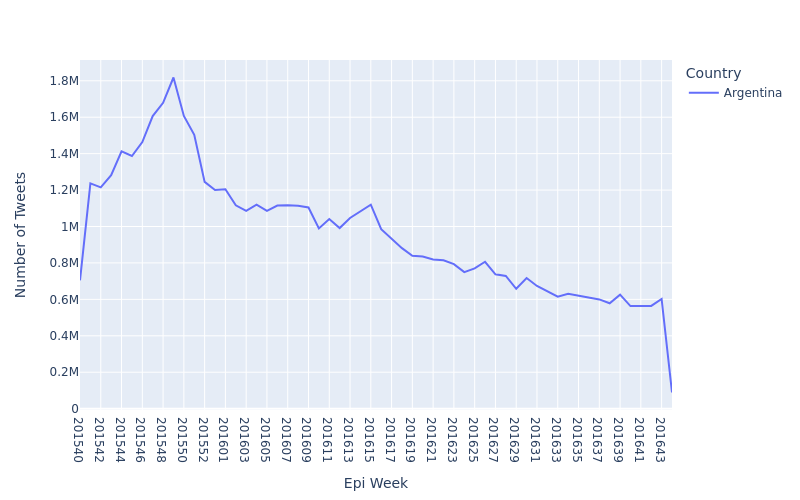
\includegraphics[width=1\textwidth]{images/geotagged_tweets_argentina_epi_week.png}
    
    \caption{Distribution of Geotagged Tweets with Argentina}
    \label{fig:geotagged-tweets-argentina-epi-week}
\end{figure}

\subsection{USA}

By considering {\fontfamily{qcr}\selectfont place\_name}, the the most commonly geotagged locations in tweets in USA were found (see Table \ref{table:mentioned-argentina}(a). Similarly, the most commonly geotagged locations by users in USA are shown in Table \ref{table:mentioned-argentina}(b).

\begin{table}
\centering
\begin{subtable}[c]{0.5\textwidth}
\centering
    \begin{tabular}{|c|c|c|}
    \hline
    Location & Number of Tweets & Proportion \\
    \hline
    Manhattan & 13989 & 0.091516 \\
    United States & 13751 & 0.089959 \\
    New York & 11383 & 0.074468 \\
    Florida & 10991 & 0.071903 \\
    Alaska & 9713 & 0.063543 \\
    Miami Beach & 9235 & 0.060416 \\
    California & 7967 & 0.052120 \\
    Miami & 4486 & 0.029347 \\
    Buenos Aires & 3165 & 0.020705 \\
    North Carolina & 3124 & 0.020437 \\
    Orlando & 2929 & 0.019162 \\
    Paterson & 2487 & 0.016270 \\
    Los Angeles & 2411 & 0.015773 \\
    Nevada & 2279 & 0.014909 \\
    Brooklyn & 2128 & 0.013921 \\
    Hawaii & 2045 & 0.013378 \\
    Washington & 1967 & 0.012868 \\
    San Francisco & 1779 & 0.011638 \\
    Hollywood & 1603 & 0.010487 \\
    Oklahoma & 1331 & 0.008707 \\
    Other & 42858 & 0.280378 \\
    \hline
    \end{tabular}
\subcaption{in Tweets}
\end{subtable}

\begin{subtable}[c]{0.5\textwidth}
\centering
    \begin{tabular}{|c|c|c|}
    \hline
    Location & Number of Tweets & Proportion \\
    \hline
    Florida & 1294 & 0.076855 \\
    Miami Beach & 1226 & 0.072816 \\
    Manhattan & 1040 & 0.061769 \\
    Miami & 946 & 0.056186 \\
    Orlando & 709 & 0.042110 \\
    New York & 417 & 0.024767 \\
    Los Angeles & 389 & 0.023104 \\
    United States & 350 & 0.020788 \\
    Brooklyn & 257 & 0.015264 \\
    Queens & 227 & 0.013482 \\
    San Francisco & 196 & 0.011641 \\
    California & 192 & 0.011403 \\
    Hollywood & 163 & 0.009681 \\
    Sunny Isles Beach & 163 & 0.009681 \\
    Paradise & 161 & 0.009562 \\
    Washington & 156 & 0.009265 \\
    Fort Lauderdale & 156 & 0.009265 \\
    Las Vegas & 152 & 0.009028 \\
    Doral & 129 & 0.007662 \\
    Chicago & 118 & 0.007008 \\
    Other & 8396 & 0.498664 \\
    \hline
    \end{tabular}
\caption{by Users}
\end{subtable}
\caption{Most Commonly Geotagged Locations in USA}
\label{table:geotagged-usa}
\end{table}



\begin{figure}[H]
    \centering
    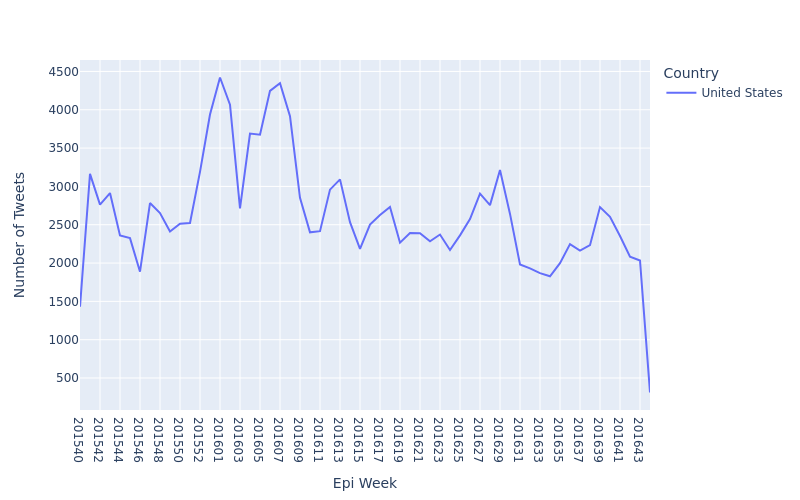
\includegraphics[width=1\textwidth]{images/geotagged_tweets_usa_epi_week.png}
    
    \caption{Distribution of Tweets Geotagged with USA}
    \label{fig:geotagged-tweets-usa-epi-week}
\end{figure}

\subsection{Brazil}

By considering {\fontfamily{qcr}\selectfont place\_name}, the the most commonly geotagged locations in tweets in Brazil were found (see Table \ref{table:mentioned-argentina}(a). Similarly, the most commonly geotagged locations by users in Brazil are shown in Table \ref{table:mentioned-argentina}(b).


\begin{table}
\centering
\begin{subtable}[c]{0.5\textwidth}
\centering
    \begin{tabular}{|c|c|c|}
    \hline
    Location & Number of Tweets & Proportion \\
    \hline
    Florianópolis & 23620 & 0.183489 \\
    Rio de Janeiro & 17070 & 0.132606 \\
    Bombinhas & 12285 & 0.095435 \\
    Ananindeua & 8702 & 0.067600 \\
    Balneário Camboriú & 5449 & 0.042330 \\
    Sao Paulo & 5069 & 0.039378 \\
    Foz do Iguaçu & 4787 & 0.037187 \\
    Itapema & 4393 & 0.034126 \\
    Armação dos Búzios & 2785 & 0.021635 \\
    Ipanema & 2399 & 0.018636 \\
    Cuiabá & 1796 & 0.013952 \\
    Porto Alegre & 1766 & 0.013719 \\
    São Vicente & 1151 & 0.008941 \\
    Natal & 1087 & 0.008444 \\
    São Sebastião & 1082 & 0.008405 \\
    Torres & 1032 & 0.008017 \\
    Mata de São João & 1014 & 0.007877 \\
    Rio Grande do Sul & 909 & 0.007061 \\
    Porto Seguro & 892 & 0.006929 \\
    Salvador & 892 & 0.006929 \\
    Other & 29667 & 0.230464 \\
    \hline
    \end{tabular}
\subcaption{in Tweets}
\end{subtable}

\begin{subtable}[c]{0.5\textwidth}
\centering
    \begin{tabular}{|c|c|c|}
    \hline
    Location & Number of Tweets & Proportion \\
    \hline
    Florianópolis & 1140 & 0.096178 \\
    Rio de Janeiro & 1032 & 0.087067 \\
    Foz do Iguaçu & 701 & 0.059141 \\
    Bombinhas & 627 & 0.052898 \\
    Balneário Camboriú & 464 & 0.039146 \\
    Sao Paulo & 383 & 0.032312 \\
    Armação dos Búzios & 296 & 0.024973 \\
    Guarulhos & 285 & 0.024045 \\
    Itapema & 283 & 0.023876 \\
    Santa Catarina & 166 & 0.014005 \\
    São Gabriel & 159 & 0.013414 \\
    Uruguaiana & 137 & 0.011558 \\
    Torres & 128 & 0.010799 \\
    Salvador & 126 & 0.010630 \\
    Porto Seguro & 123 & 0.010377 \\
    Porto Alegre & 119 & 0.010040 \\
    Angra dos Reis & 117 & 0.009871 \\
    Brazil & 115 & 0.009702 \\
    Garopaba & 107 & 0.009027 \\
    Brasília & 103 & 0.008690 \\
    Other & 5242 & 0.442251 \\
    \hline
    \end{tabular}
\caption{by Users}
\end{subtable}
\caption{Most Commonly Geotagged Locations in Brazil}
\label{table:geotagged-brazil}
\end{table}


\begin{figure}[H]
    \centering
    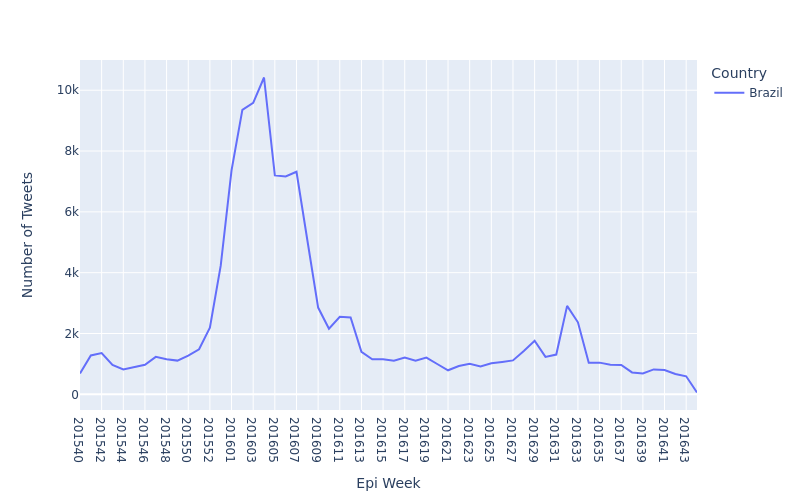
\includegraphics[width=1\textwidth]{images/geotagged_tweets_brazil_epi_week.png}
    
    \caption{Distribution of Tweets Geotagged with Brazil}
    \label{fig:geotagged-tweets-brazil-epi-week}
\end{figure}

\pagebreak

\section{Mentioned}

Since some tweets mentioned more than one location, the total number of toponyms (LOC mentions) was 9,017,197 (tweets duplicated to capture all mentions), compared to 7,269,062 mentioned tweets. Similarly, the number of geoparsed toponyms was 4,139,502, compared to 3,462,888 geoparsed tweets. This section explores geoparsed toponyms, as they have the most location information associated with them.

514284 locations were disregarded (corresponding to 828684 tweets), 46952 were kept (corresponding to 7204497 tweets). 

 
\subsection{Granularity}

Figure \ref{fig:mention-pie} shows the granularity of geoparsed toponyms. 

\begin{figure}[H]
    \centering
    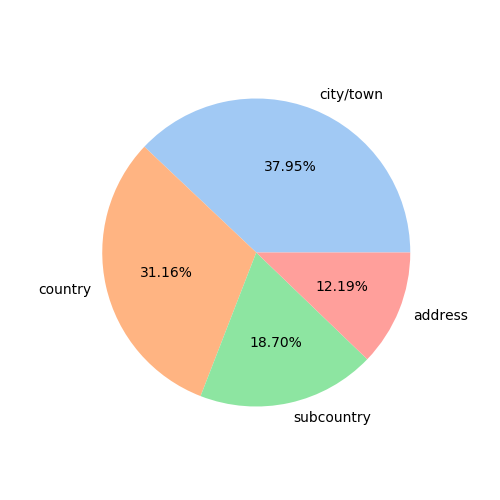
\includegraphics[width=0.5\textwidth]{images/granularity.png}
    
    \caption{Granularity of Mentions}
    \label{fig:mention-pie}
\end{figure}

%Table \ref{tab:granularity} shows the tweet granularity of mentions within tweets, excluding those that did not correspond to a location in Geolocator API.
The "subcountry" granularity was used to describe geoparsed toponyms that contained a county, province, region, district etc. but did not contain a city/town. "Address" was used to describe a toponym that had a specific street-level address.

\begin{comment}
\begin{table}[H]
  \centering
  \begin{tabular}{|c|c|c|}
    \hline
    %& \multicolumn{2}{c|}{\textbf{Mention}} & \multicolumn{2}{c|}{\textbf{Mention Only}} \\
    %\cline{3-6}
    \textbf{Granularity} & \textbf{Number of Tweets} & \textbf{Proportion}\\
    \hline
    city/town &	1570867 &	0.379482 \\
    \hline
    country &	1290046 &	0.311643 \\
    \hline
    subcountry &	773963 &	0.186970 \\
    address & 	504626 & 	0.121905 \\
    \hline
  \end{tabular}
  \caption{Geoparsed Toponym Granularity}
  \label{tab:granularity}
\end{table}
\end{comment}

\subsection{All Countries}

To understand which countries were mentioned most often in tweets, the number of geoparsed toponyms associated with each mentioned country was found. The top 20 countries mentioned in tweets are shown in Table \ref{table:mentioned-countries}(a).

For each user, a list of countries they mentioned during the relevant time period was found (using location information from geoparsed toponyms). This information was aggregated by finding the number of users that mentioned each country. Table \ref{table:mentioned-countries}(b) shows the top 20 countries mentioned most often by users.

\begin{table}[H]
\begin{subtable}[c]{0.5\textwidth}
\centering
\begin{tabular}{|c|c|c|}
\hline
    \textbf{Location} & \textbf{Count} & \textbf{Proportion} \\
    \hline
    Argentina & 2157309.0 & 0.521152 \\
    USA & 532081.0 & 0.128537 \\
    Brazil & 131189.0 & 0.031692 \\
    Chile & 97427.0 & 0.023536 \\
    Spain & 96466.0 & 0.023304 \\
    Italy & 94749.0 & 0.022889 \\
    France & 71005.0 & 0.017153 \\
    Mexico & 69886.0 & 0.016883 \\
    United States & 67970.0 & 0.016420 \\
    Colombia & 48817.0 & 0.011793 \\
    Venezuela & 40560.0 & 0.009798 \\
    Uruguay & 39403.0 & 0.009519 \\
    UK & 38552.0 & 0.009313 \\
    Puerto Rico & 28763.0 & 0.006948 \\
    Japan & 27415.0 & 0.006623 \\
    China & 25588.0 & 0.006181 \\
    Germany & 23716.0 & 0.005729 \\
    Paraguay & 22557.0 & 0.005449 \\
    Bulgaria & 21419.0 & 0.005174 \\
    Peru & 21268.0 & 0.005138 \\
    Other & 464182.0 & 0.112135 \\
    \hline
    \end{tabular}
\subcaption{in Tweets}
%\label{table:mentioned-countries-tweets}
\end{subtable}
\begin{subtable}[c]{0.5\textwidth}
\centering
\begin{tabular}{|c|c|c|}
\hline
    \textbf{Location} & \textbf{Count} & \textbf{Proportion} \\
    \hline
    Argentina & 74323 & 0.123 \\
    USA & 60282 & 0.100 \\
    Brazil & 28767 & 0.048 \\
    Italy & 27548 & 0.046 \\
    Spain & 24842 & 0.041 \\
    Chile & 22576 & 0.037 \\
    France & 22121 & 0.037 \\
    Mexico & 19505 & 0.032 \\
    United States & 14443 & 0.024 \\
    Colombia & 12920 & 0.021 \\
    UK & 12052 & 0.020 \\
    Uruguay & 10966 & 0.018 \\
    China & 10515 & 0.017 \\
    Japan & 8890 & 0.015 \\
    Germany & 8575 & 0.014 \\
    Venezuela & 8212 & 0.014 \\
    Puerto Rico & 8209 & 0.014 \\
    Australia & 8066 & 0.013 \\
    Peru & 7907 & 0.013 \\
    India & 7741 & 0.013 \\
    Other & 205642 & 0.340 \\
    \hline
    \end{tabular}
\subcaption{by Users}
\label{table:mentioned-countries}
\end{subtable}
\caption{Most Mentioned Countries}
\end{table}

To investigate temporal patterns, the number of times the top 5 countries in \ref{table:mentioned-countries}(a) (excluding Argentina) were mentioned during each epi week was found. Figure \ref{fig:mentioned-tweets-country-epi-week} shows when these countries were mentioned over time.

Similarly, the number of users mentioning the top 5 countries in \ref{table:mentioned-countries}(b) (excluding Argentina) during each epi week was found (see Figure \ref{fig:mentioned-users-country-epi-week}).

\begin{figure}[H]
    \centering
    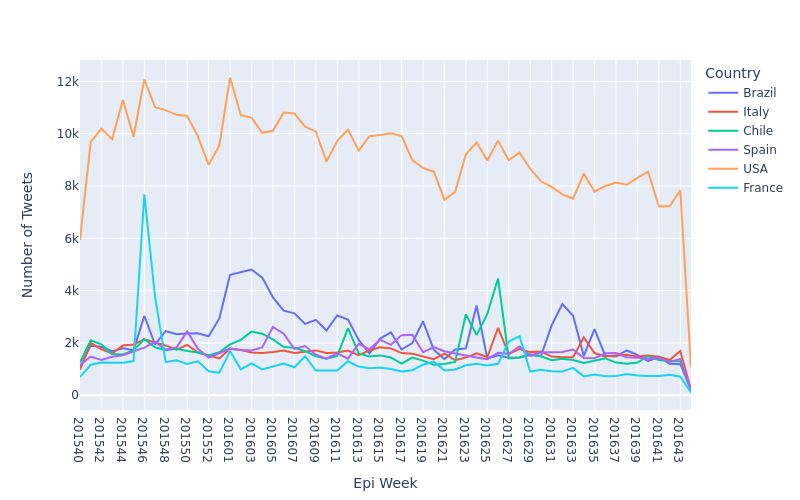
\includegraphics[width=1\textwidth]{images/mentioned_tweets_country_epi_week.png}
    
    \caption{Distribution of Top 5 Most Geotagged Countries (Tweets)}
    \label{fig:mentioned-tweets-country-epi-week}
\end{figure}

\begin{figure}[H]
    \centering
    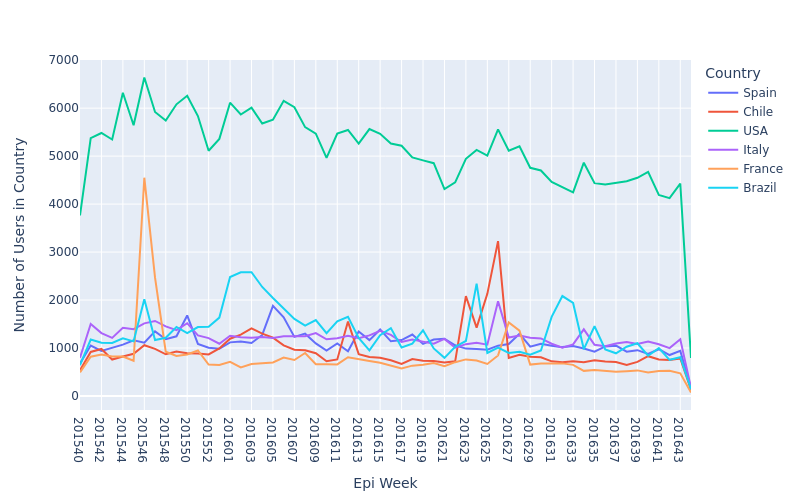
\includegraphics[width=1\textwidth]{images/mentioned_users_country_epi_week.png}
    
    \caption{Distribution of Top 5 Most Geotagged Countries (Users)}
    \label{fig:mentioned-users-country-epi-week}
\end{figure}

\subsection{Argentina}

If geoparsed toponyms contained city/town information, the most commonly mentioned cities/towns in tweets in Argentina were found (see Table \ref{table:mentioned-argentina}(a).
Similarly, the most commonly mentioned cities/towns in Argentina are shown in Table \ref{table:mentioned-argentina}(b).
Figure \ref{fig:mentioned-tweets-argentina-epi-week} shows the number of times Argentina was mentioned in tweets during each epi week.

\begin{table}
\centering
\begin{subtable}[c]{0.5\textwidth}
\centering
\begin{tabular}{|c|c|c|}
\hline
    \textbf{Location} & \textbf{Count} & \textbf{Proportion} \\
    \hline
    Rosario & 88325.0 & 0.086508 \\
    San Carlos de Bariloche & 53501.0 & 0.052400 \\
    La Plata & 46432.0 & 0.045477 \\
    Capital Department & 43428.0 & 0.042535 \\
    Mar del Plata & 42159.0 & 0.041292 \\
    Salta & 37853.0 & 0.037074 \\
    San Miguel de Tucumán & 31238.0 & 0.030595 \\
    Quilmes & 21652.0 & 0.021207 \\
    Avellaneda & 16396.0 & 0.016059 \\
    San Salvador de Jujuy & 14388.0 & 0.014092 \\
    Posadas & 12154.0 & 0.011904 \\
    San Martín & 11944.0 & 0.011698 \\
    Catamarca & 11856.0 & 0.011612 \\
    Bahía Blanca & 11609.0 & 0.011370 \\
    Av. Hipólito Yrigoyen s/n & 10619.0 & 0.010401 \\
    Ezeiza & 9584.0 & 0.009387 \\
    San Isidro & 9092.0 & 0.008905 \\
    Villa Carlos Paz & 9079.0 & 0.008892 \\
    Ushuaia & 8644.0 & 0.008466 \\
    Puerto Madero & 8583.0 & 0.008406 \\
    Other & 514462.0 & 0.503880 \\
    \hline
    \end{tabular}
\subcaption{in Tweets}
\end{subtable}

\begin{subtable}[c]{0.5\textwidth}
\centering
\begin{tabular}{|c|c|c|}
\hline
    \textbf{Location} & \textbf{Count} & \textbf{Proportion} \\
    \hline
    San Carlos de Bariloche & 15330.0 & 0.056753 \\
    Rosario & 11999.0 & 0.044421 \\
    Capital Department & 8259.0 & 0.030575 \\
    Mar del Plata & 8187.0 & 0.030309 \\
    La Plata & 7369.0 & 0.027280 \\
    Avellaneda & 5643.0 & 0.020891 \\
    Quilmes & 5566.0 & 0.020606 \\
    San Miguel de Tucumán & 5521.0 & 0.020439 \\
    Salta & 5343.0 & 0.019780 \\
    San Martín & 4137.0 & 0.015315 \\
    San Salvador de Jujuy & 3919.0 & 0.014508 \\
    Puerto Madero & 3826.0 & 0.014164 \\
    Ezeiza & 3427.0 & 0.012687 \\
    Av. Hipólito Yrigoyen s/n & 3378.0 & 0.012506 \\
    Villa Carlos Paz & 3377.0 & 0.012502 \\
    Tandil & 3027.0 & 0.011206 \\
    San Isidro & 2534.0 & 0.009381 \\
    Santiago del Estero & 2434.0 & 0.009011 \\
    Recoleta & 2293.0 & 0.008489 \\
    Catamarca & 2249.0 & 0.008326 \\
    Other & 162302.0 & 0.600851 \\
    \hline
    \end{tabular}
\caption{by Users}
\end{subtable}
\caption{Most Commonly Mentioned cities/towns in Argentina}
\label{table:mentioned-argentina}
\end{table}

\begin{figure}[H]
    \centering
    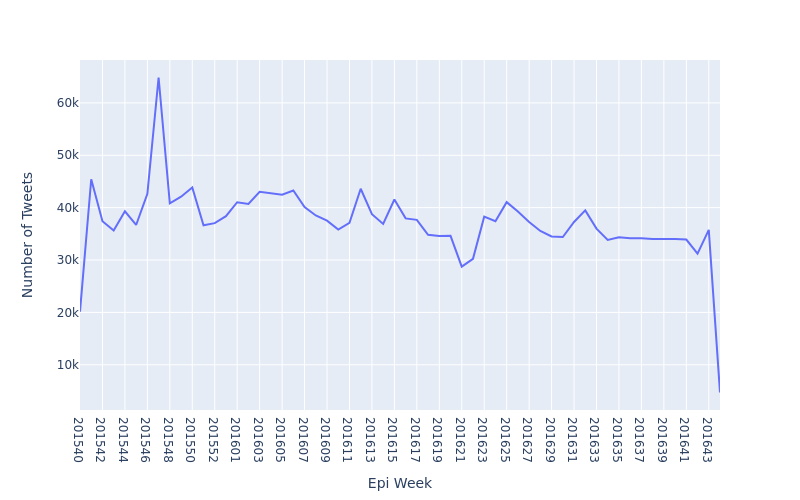
\includegraphics[width=1\textwidth]{images/mentioned_tweets_argentina_epi_week.png}
    
    \caption{Tweets Mentioning Argentina Over Time}
    \label{fig:mentioned-tweets-argentina-epi-week}
\end{figure}

\subsection{USA}

If geoparsed toponyms contained city/town information, the most commonly mentioned cities/towns in tweets in USA were found (see Table \ref{table:mentioned-argentina}(a).
Similarly, the most commonly mentioned cities/towns in USA are shown in Table \ref{table:mentioned-argentina}(b).
Figure \ref{fig:mentioned-tweets-argentina-epi-week} shows the number of times USA was mentioned in tweets during each epi week.

USA was chosen because it was the second most mentioned country from previous analysis.

\begin{table}
\centering
\begin{subtable}[c]{0.5\textwidth}
\centering
\begin{tabular}{|c|c|c|}
\hline
    \textbf{Location} & \textbf{Count} & \textbf{Proportion} \\
    \hline
    Santa Fe & 48704.0 & 0.181962 \\
    New York & 22526.0 & 0.084159 \\
    Miami & 17731.0 & 0.066244 \\
    Santa Cruz & 13279.0 & 0.049611 \\
    Santa Rosa & 10286.0 & 0.038429 \\
    Los Angeles & 9557.0 & 0.035706 \\
    San Francisco & 9056.0 & 0.033834 \\
    Chicago & 8632.0 & 0.032250 \\
    San Rafael & 4986.0 & 0.018628 \\
    Atlanta & 4765.0 & 0.017802 \\
    Brooklyn & 4664.0 & 0.017425 \\
    Orlando & 4370.0 & 0.016327 \\
    San Fernando & 4284.0 & 0.016005 \\
    San Nicolas Island & 3950.0 & 0.014758 \\
    Las Vegas & 3624.0 & 0.013540 \\
    Miramar & 2887.0 & 0.010786 \\
    Miami Beach & 2853.0 & 0.010659 \\
    San Jose & 2744.0 & 0.010252 \\
    Martinez & 2544.0 & 0.009505 \\
    Buena & 2461.0 & 0.009195 \\
    Other & 81363.0 & 0.303979 \\
    \hline
    \end{tabular}
\subcaption{in Tweets}
\end{subtable}

\begin{subtable}[c]{0.5\textwidth}
\centering
\begin{tabular}{|c|c|c|}
\hline
    \textbf{Location} & \textbf{Count} & \textbf{Proportion} \\
    \hline
    Santa Fe & 8523.0 & 0.094506 \\
    Miami & 7605.0 & 0.084327 \\
    New York & 5883.0 & 0.065233 \\
    Los Angeles & 3586.0 & 0.039763 \\
    Santa Cruz & 2889.0 & 0.032034 \\
    Chicago & 2870.0 & 0.031823 \\
    Santa Rosa & 2488.0 & 0.027588 \\
    Orlando & 2334.0 & 0.025880 \\
    San Francisco & 2232.0 & 0.024749 \\
    Alta & 1864.0 & 0.020669 \\
    Las Vegas & 1791.0 & 0.019859 \\
    Buena & 1546.0 & 0.017143 \\
    Islandia & 1429.0 & 0.015845 \\
    Brooklyn & 1264.0 & 0.014016 \\
    Miramar & 1153.0 & 0.012785 \\
    Atlanta & 1151.0 & 0.012763 \\
    San Pablo & 1140.0 & 0.012641 \\
    San Jose & 1118.0 & 0.012397 \\
    San Nicolas Island & 1115.0 & 0.012363 \\
    San Antonio & 1110.0 & 0.012308 \\
    Other & 37094.0 & 0.411310 \\
    \hline
    \end{tabular}
\caption{by Users}
\end{subtable}
\caption{Most Commonly Mentioned cities/towns in USA}
\label{table:mentioned-usa}
\end{table}

\begin{figure}[H]
    \centering
    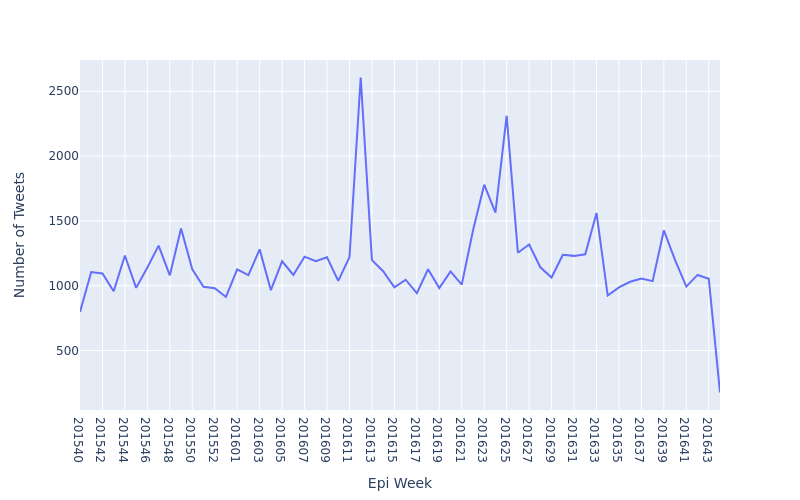
\includegraphics[width=1\textwidth]{images/mentioned_tweets_us_epi_week.png}
    
    \caption{Tweets Mentioning USA Over Time}
    \label{fig:mentioned-tweets-us-epi-week}
\end{figure}

\subsection{Brazil}

If geoparsed toponyms contained city/town information, the most commonly mentioned cities/towns in tweets in USA were found (see Table \ref{table:mentioned-argentina}(a).
Similarly, the most commonly mentioned cities/towns in USA are shown in Table \ref{table:mentioned-argentina}(b).
Figure \ref{fig:mentioned-tweets-argentina-epi-week} shows the number of times USA was mentioned in tweets during each epi week.

Brazil was chosen because it was third most mentioned country and it has the highest incidence of dengue virus in the Americas.

\begin{table}
\centering
\begin{subtable}[c]{0.5\textwidth}
\centering
\begin{tabular}{|c|c|c|}
\hline
    \textbf{Location} & \textbf{Count} & \textbf{Proportion} \\
    \hline
    Brasília - Brasilia & 6431.0 & 0.164830 \\
    Ananindeua & 5934 & 0.152091 \\
    Rio de Janeiro & 4205.0 & 0.107776 \\
    São Paulo & 2454.0 & 0.062897 \\
    Florianópolis & 2050.0 & 0.052543 \\
    Manaus & 926.0 & 0.023734 \\
    Armação dos Búzios & 668.0 & 0.017121 \\
    Av. Brasil & 571.0 & 0.014635 \\
    Foz do Iguaçu & 539.0 & 0.013815 \\
    State of São Paulo & 510.0 & 0.013072 \\
    Rio de Janeiro - RJ & 506.0 & 0.012969 \\
    Santa Catarina & 467.0 & 0.011969 \\
    São Paulo - SP & 455.0 & 0.011662 \\
    Porto Alegre & 432.0 & 0.011072 \\
    Belo Horizonte & 403.0 & 0.010329 \\
    Praia de Canasvieiras & 400.0 & 0.010252 \\
    Curitiba & 387.0 & 0.009919 \\
    SC & 354.0 & 0.009073 \\
    Palmas & 352.0 & 0.009022 \\
    Maracanã & 328.0 & 0.008407 \\
    Other & 10323.0 & 0.264584 \\
    \hline
    \end{tabular}
\subcaption{in Tweets}
\end{subtable}

\begin{subtable}[c]{0.5\textwidth}
\centering
\begin{tabular}{|c|c|c|}
\hline
    \textbf{Location} & \textbf{Count} & \textbf{Proportion} \\
    \hline
    Rio de Janeiro & 1753.0 & 0.121770 \\
    Brasília - Brasilia & 1724.0 & 0.119755 \\
    Florianópolis & 876.0 & 0.060850 \\
    São Paulo & 860.0 & 0.059739 \\
    Manaus & 782.0 & 0.054321 \\
    Av. Brasil & 369.0 & 0.025632 \\
    Rio de Janeiro - RJ & 309.0 & 0.021464 \\
    State of São Paulo & 297.0 & 0.020631 \\
    Armação dos Búzios & 288.0 & 0.020006 \\
    Palmas & 269.0 & 0.018686 \\
    Maracanã & 251.0 & 0.017435 \\
    Foz do Iguaçu & 242.0 & 0.016810 \\
    Porto Alegre & 233.0 & 0.016185 \\
    Santa Catarina & 217.0 & 0.015074 \\
    Belo Horizonte & 185.0 & 0.012851 \\
    Ipanema & 167.0 & 0.011600 \\
    State of Santa Catarina & 165.0 & 0.011462 \\
    Praia de Canasvieiras & 164.0 & 0.011392 \\
    Curitiba & 156.0 & 0.010836 \\
    Praia dos Ingleses & 153.0 & 0.010628 \\
    Other & 4936.0 & 0.342873 \\
    \hline
    \end{tabular}
\caption{by Users}
\end{subtable}
\caption{Most Commonly Mentioned cities/towns in Brazil}
\label{table:mentioned-brazil}
\end{table}

\begin{figure}[H]
    \centering
    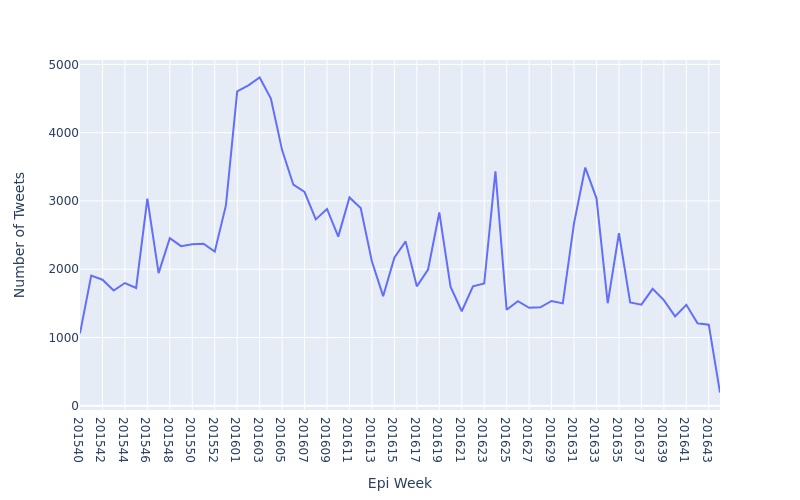
\includegraphics[width=1\textwidth]{images/mentioned_tweets_br_epi_week.png}
    
    \caption{Tweets Mentioning Brazil Over Time}
    \label{fig:mentioned-tweets-br-epi-week}
\end{figure}

\pagebreak
\section{Geotagged \& Mentioned}

Where a tweet had both a geoparsed set of coordinates and a geotagged set of coordinates, the geodesic distance was calculated in kilometres.

A subset of these tweets had more than one geoparsed set of coordinates. These tweets were called Duplicates. The subset of tweets with a unique geoparsed set of coordinates was called Non-Duplicates. 

Table \ref{table:summary-distances} shows summary statistics for distances between geotagged coordinates and mentioned (geoparsed) coordinates for all the tweets with geoparsed and geotagged locations, as well as subsets Duplicates and Non-Duplicates.

\begin{table}[H]
    \centering
    \begin{tabular}{|l|c|c|c|}
    \hline
    Metric & All & Duplicates & Non-Duplicates \\
    \hline
    MdnED & 479.11 & 142.58 & 631.54 \\
    MED & 2708.79 & 1977.22 & 3477.69 \\
    Accuracy@0.1 & 0.031 & 0.033 & 0.028 \\
    Accuracy@0.5 & 0.074 & 0.080 & 0.066 \\
    Accuracy@1 & 0.132 & 0.140 & 0.124 \\
    Accuracy@5 & 0.254 & 0.306 & 0.200 \\
    Accuracy@10 & 0.297 & 0.358 & 0.233 \\
    Accuracy@25 & 0.358 & 0.421 & 0.292 \\
    Accuracy@50 & 0.380 & 0.450 & 0.307 \\
    Accuracy@100 & 0.404 & 0.484 & 0.321 \\
    Accuracy@161 & 0.427 & 0.516 & 0.333 \\
    Accuracy@1000 & 0.670 & 0.740 & 0.597 \\
    \hline
    \end{tabular}
    \caption{Summary of Distances}
    \label{table:summary-distances}
\end{table}



are these kilometers? explain the difference between duplicate and non-duplicate in the table caption

\begin{figure}[H]
    \centering
    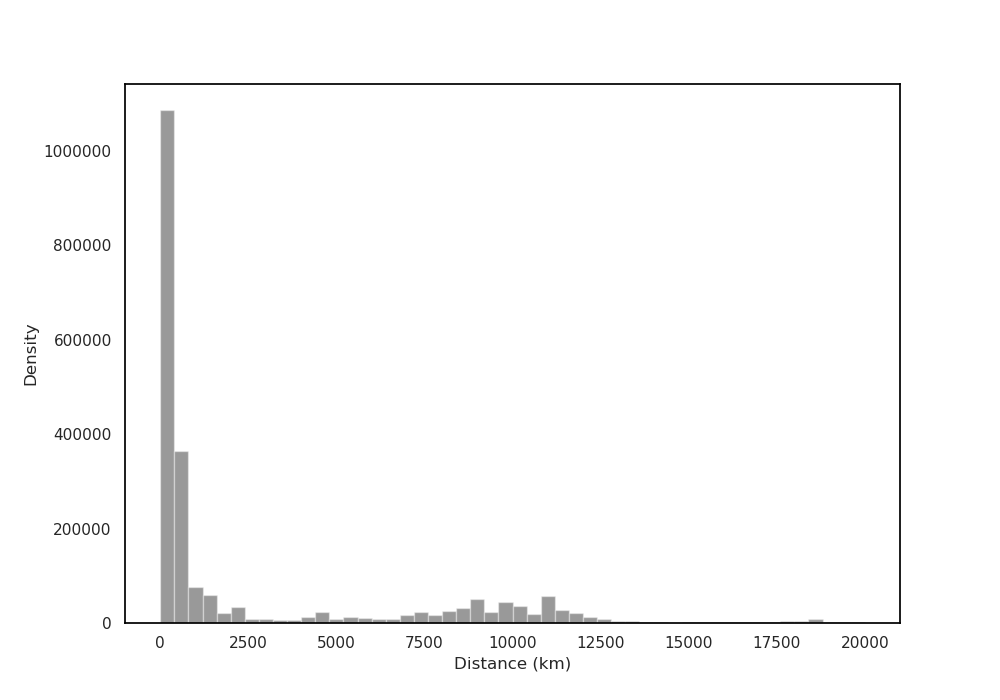
\includegraphics[width=1\textwidth]{images/distance_frequency.png}
    
    \caption{Distribution of Distances}
    \label{fig:distribution-distances}
\end{figure}

Figure \ref{fig:distribution-distances} shows distribution of all distances (not taking into account that some tweets have duplicate locations).

\begin{figure}[H]
    \centering
    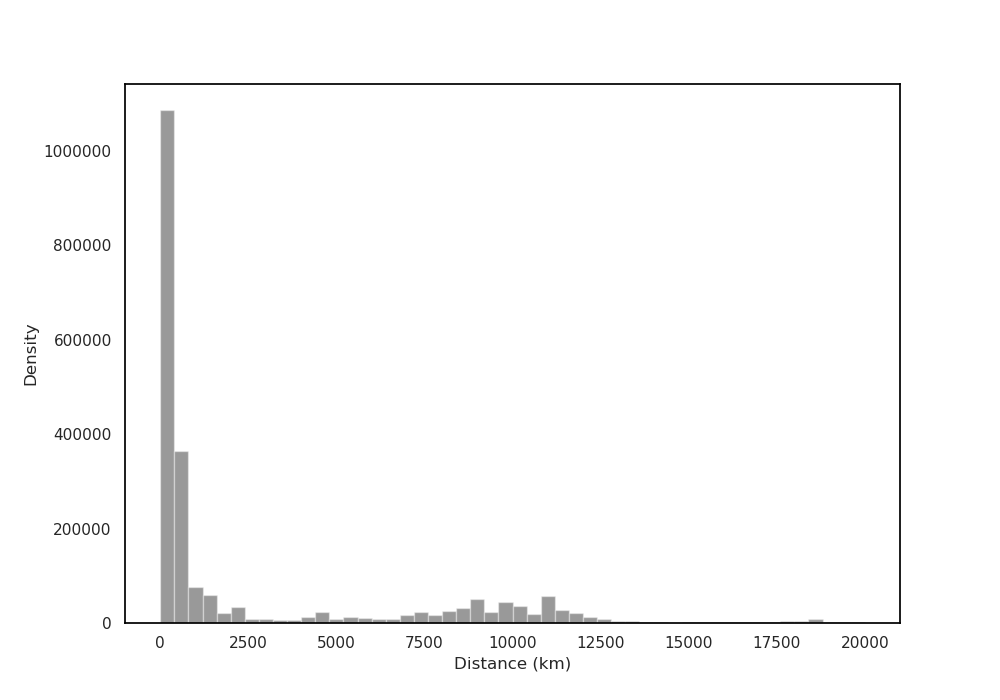
\includegraphics[width=1\textwidth]{images/distance_frequency.png}
    
    \caption{Distribution of Distances}
    \label{fig:distance-frequency}
\end{figure}

482,741 of tweets had a geoparsed country and a geotagged country that was the same, and in 868,020 tweets the geoparsed and geotagged tweets were different (considering duplicates due to multiple geoparsed toponyms per tweet).

\subsection{If Argentina was mentioned, where were the geotags?}

444333 of the geotags in this subset of the data corresponded to Argentina, corresponding to over 96\%. So Argentina was filtered out to get a better understanding of geotagged countries.

\begin{table}[H]
\centering
\begin{tabular}{lcc}
\hline
Country & Counts & Proportion \\
\hline
Brazil & 2454 & 0.136409 \\
USA & 2344 & 0.130295 \\
Chile & 1476 & 0.082046 \\
Uruguay & 874 & 0.048583 \\
Mexico & 682 & 0.037910 \\
Spain & 623 & 0.034630 \\
Peru & 456 & 0.025347 \\
Paraguay & 445 & 0.024736 \\
Italy & 363 & 0.020178 \\
France & 337 & 0.018733 \\
Colombia & 335 & 0.018621 \\
United Kingdom & 315 & 0.017510 \\
Ecuador & 262 & 0.014564 \\
Dominican Republic & 221 & 0.012285 \\
Japan & 220 & 0.012229 \\
Bolivia & 209 & 0.011618 \\
Canada & 195 & 0.010839 \\
Germany & 171 & 0.009505 \\
Indonesia & 165 & 0.009172 \\
Other & 5679 & 0.315675 \\
\hline
\end{tabular}
\caption{Country Counts and Proportions}
\label{tab:distances-argentina-mentioned}
\end{table}


\subsection{If the geotag is Argentina, what are the mentions?}

Again, Argentina was filtered out for the same reason as above.

\begin{table}[H]
\centering
\begin{tabular}{lcc}
\hline
Country & Counts & Prop \\
\hline
USA & 126,511 & 0.267 \\
Brazil & 28,233 & 0.060 \\
Italy & 27,680 & 0.058 \\
Spain & 25,060 & 0.053 \\
Chile & 20,070 & 0.042 \\
Mexico & 18,613 & 0.039 \\
France & 16,267 & 0.034 \\
United States & 11,555 & 0.024 \\
Colombia & 11,449 & 0.024 \\
Uruguay & 8,679 & 0.018 \\
Venezuela & 8,553 & 0.018 \\
UK & 7,694 & 0.016 \\
Puerto Rico & 7,634 & 0.016 \\
Peru & 5,891 & 0.012 \\
Bulgaria & 5,789 & 0.012 \\
China & 5,726 & 0.012 \\
Japan & 5,562 & 0.012 \\
Paraguay & 5,325 & 0.011 \\
Germany & 5,126 & 0.011 \\
Other & 116,800 & 0.247 \\
\hline
\end{tabular}
\caption{Argentina Geotagged}
\label{distances-argentina-geotagged}
\end{table}

The top 30 geotagged countries and top 30 geoparsed countries were found, and their intersection was found. For the resulting 20 countries, a heatmap was produced. 

\begin{figure}[H]
    \centering
    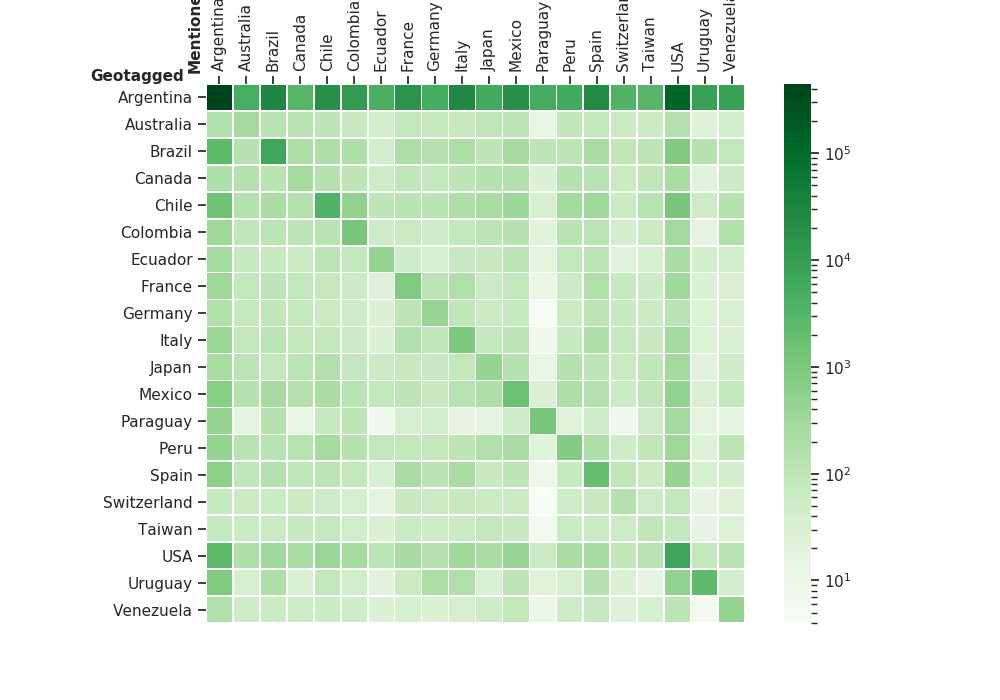
\includegraphics[width=1\textwidth]{images/distance-heatmap.png}
    
    \caption{Number of Tweets With Geotagged Country vs Mentioned (Geoparsed) Country Heatmap}
    \label{fig:distance-heatmap}
\end{figure}


 
\chapter{Discussion} %W7

%There is no mention of the specific limitations of the second approach used to collect tweets, which was based on filtering users based on language and location. It would be helpful to address potential issues with this method, such as whether it could exclude certain demographics or whether there could be biases introduced by language filtering.

%There is no mention of how the NER model was trained and what kind of data it was trained on. This information could help explain the misclassifications observed and provide insight into how to improve the model's accuracy.

%It would be helpful to provide more information on how the Google Geocoding API works and what factors could affect its accuracy. This information could help explain the low success rate of geoparsing and provide insights into how to improve it.

\section{How can tweets be collected from a geographically-defined set of users?}

The traditional method of collecting tweets (Section \ref{approach-1}) did not yield a sufficient volume of tweets and the distribution of tweets was not what was expected. This was likely due to how the search function works on Twitter.

The second approach (Section \ref{approach-2}) yielded much more promising results. It is estimated that 1\% of tweets are geotagged, so the data collection method used yielding 30\% which was certainly fortuitous. This was likely because the usernames were extracted based on whether the user geotagged Argentina in their tweet, so the users were more likely to geotag their location.

It is unknown how Twitter determines where a tweet came from, so collecting tweets based on location-based search criteria can be unreliable. It could be a combination of IP address, user location and geotag. With public geotagged tweets, it is unambiguous what the user claimed as their location (as there is seemingly no way to know the ground truth from available data).

The distribution of countries geotagged in tweets and geotagged by users make sense, since Argentina was geotagged most often and over half of the other 20 most mentioned countries in Table \ref{table:geotagged-countries} were from countries in the Americas. The spike in tweets geotagged with Brazil seen between 1st and 9th epi weeks corresponds to the Brazilian Carnival, celebrated in February. The United States is geotagged most often in general (apart from Argentina), however it would be interesting to investigate whether there are trends within specific locations (geotags in New York, Los Angeles, Miami, etc. and whether these correspond to tourist seasons). 

Choosing a geographically defined set of users by using a broad commonality like language spoken (e.g. Spanish), then filtering based on country, seems to result in a higher volume of higher quality tweets (more geotagged) than using geographical search parameters alone. This also means our data likely has more Argentinian and Central/South American residents than tourists due to the language filter.

Further data analysis can provide more insights into the geotagged data. Here are some ways in which the data can be further analyzed:
\begin{description}
    \item[Types of Tweets] Analyzing the content of geotagged tweets can provide insights into the types of topics and conversations that are prevalent in different locations. For example, analyzing the use of hashtags in geotagged tweets can reveal the most commonly used hashtags in different locations, and this can be used to identify the topics that are currently popular in those locations. Additionally, what proportions of tweets contain only links? How many mention other users?
    \item[Types of Users] The geotagged data can be used to identify the types of users who are active in different locations. For example, analyzing the frequency of tweets by different users can help identify frequent tweeters, while analyzing the use of links in tweets can identify event promoters and organizations.
    \item[Real People vs. Spam Accounts] Analyzing the patterns of tweets can help identify which accounts are likely to be spam accounts or bots, and which are likely to be real people. For example, accounts that tweet very frequently or use very similar phrasing in their tweets may be more likely to be bots.
    \item[Username Collection] Analyzing the usernames collected over three days can reveal whether there are any patterns or trends in the types of users who are active on specific days of the week. This can be used to identify the best days for collecting geotagged data in order to get the most representative sample.
    \item[Visits to Argentina] Argentina was geotagged most often at the end of 2015, after which there was a steady decline. What caused this? Might tweeters be most active around that time?
\end{description}

\section{Can NLP be used to derive location information from tweet content?}

For decades, NLP has been used to extract various entities, but the transformer architecture, which is relatively new and produces similar results for NER, has been gaining popularity (\cite{vaswani_attention_2017}). In the total tweets collected, less than 4\% mentioned a location. Upon further inspection, it was discovered that some of the mentioned locations were misclassified by the BERT NER model as organizations. This may be due to the difficulty of extracting named entities from short texts like tweets.

Out of all the tweets collected, only 1.65\% were successfully geoparsed through the Google Geocoding API. Given the misclassifications in NER, it would be interesting to investigate whether a gazetteer would be more effective than BERT followed by the Geocoding API.

Argentina was mentioned in over 52\% of tweets, whereas if the mentions are aggregated by user, Argentina was mentioned only 12\% of the time. This suggests that more users are mentioning Argentina more often than any other country.

When investigating mentions in tweets, a similar spike in mentions of Brazil was observed, but it was much smaller compared to the geotags of Brazil. This may be due to mentions being a smaller subset of tweets, and it may not necessarily mean that the location was mentioned in the tweet. It could also be because the BERT NER model did not identify the location, or the Google Geoparser API is incorrectly mapping the location.

Additionally, the Google Geocoding API may also be inaccurately disambiguating locations, such as Cordoba in Spain versus Argentina. It is also unknown how many locations have two names, such as "USA" and "United States". The inaccuracy may also be due to the fact that the tweets were mostly in Spanish, and the Google Geocoding API may not work as well in disambiguating those. Previous studies have suggested that a multilingual gazetteer may work better, as seen in \cite{wang_enhancing_2019}.

During the analysis of mentioned tweets, the locations "United States" and "USA" were not aggregated, and the analysis had to be halted due to technical restrictions of the cloud computing platform used.

While the frequency of geotags of Argentina declined over time, the mentions remained mostly constant over the chosen time period, with a few spikes.

Initially, it was hypothesized that there would be more tweets with mentioned locations than geotagged tweets, but this was not the case likely due to the data collection method. While mentioned locations were more granular by default, they are likely less useful than the geotagged tweets themselves due to there being fewer of them and potentially further away from the ground truth of where the user was (as indicated by the proportionally more mentions of "USA" than geotags of "USA").

Further analysis could be done to investigate how many other countries have more than one location name, and whether mentions of organizations and people indicate anything about the content of the tweets and user segregation.

\section{Are geotagged locations and mentioned locations measuring the same thing?}

The percentage of tweets that had both a geotag and a geoparsed mention was very low at 0.94\%. However, this was the only way to compare the two. Previous research considered geotags to be the ground truth \cite{wang_enhancing_2019}, but this must be investigated further before this data is used for investigating regional travel patterns.

The reason for the discrepancy could be that people are tweeting about a location that they are not actually in. For example, 96\% of tweets that had both a geotag and a mention were about Argentina, but this is significantly lower than the accuracy of geotags within 1000km. This suggests that even if a tweet has a geotag and a mention with the same country, they are likely not in the same location (at least 1000km apart).

Overall, geotags and mentions are not always the same, as only 36\% of geoparsed geotagged tweets had the same country. Over 64\% of tweets did not even have the same country, and less than 50\% of coordinates were within 100km of each other.

The granularity of geotagged tweets could not be investigated, but comparing tweets with both a geotag and a geoparsed location within a small radius could reveal the types of locations people visit and the purpose of their travel.

Further analysis could aggregate tweets from each user for each week and provide more context for extracting entities and locations. This could help distinguish between when a user is talking about a place or talking about being in that place.

% distribution of geotagged and mentioned countries (tweets vs users)
%The distribution of countries in Figures 4.3 and 4.4 closely follow each other, meaning the effect of any biases due to people spamming tweets is minimal. This is similar to Figures 4.8 and 4.9. The spike for geotagged tweets in Brazil is higher than mentioned tweets, which suggests more people geotagged Brazil than mentioned it in their tweets. This was likely about Carnaval, and could either be due to Geocoding API not mapping references to carnaval correctly or people genuinely geotagging more than mentioning Brazil.

% Is it because Google API isn't the best choice for accurately geoparsing NLP toponyms?
% Is it because some of these tools were developed for use in English?
% You can also suggest ideas for improvement or further investigation: maybe the geotags need to be geoparsed first.
% Maybe another gazetteer would be better.
% Maybe all tweets from a user in a week need to be put together so NLP has a larger body of text to read.
% Maybe user information could be combined with the tweet text in some way.
% Maybe a more interesting question in the future is if NLP can tell the difference between a user talking about a place versus talking about where they are.
% What might NLP need to make that work.
% I'm not saying you have to do any of these, but a good discussion section talks about the limitations of the work that's been done, possible explanations for what has been found, and ideas for next steps. 

% Don't stress about not being able to relate any of this to dengue - remember you are working to see if this method works in general. I think you have found that this is a really complex problem and "solving" it is probably beyond the scope of your honours project. But you have found a lot of helpful and interesting things about working with this type of data!!


 
\chapter{Conclusion}
Collecting tweets from a geographically-defined set of users can be a challenging task due to the unreliable nature of Twitter's location-based search criteria. However, using a language filter based on a broad commonality like Spanish, then filtering based on country, seems to yield a higher volume of higher quality tweets, especially if one is interested in analyzing the views of local residents.

While the geoparsing process using BERT NER and Google Geocoding API shows promise, it is still unclear why it has not yielded better results in the given context. This method has its limitations, and more research is needed to improve its accuracy. Additionally, the small number of locations mentioned in the tweets compared to the total number of tweets and geotagged tweets indicates that they may not be of much use in practical applications.

It is essential to note that geoparsed and geotagged locations are not interchangeable, as the NLP methods used in geoparsing do not always accurately capture the intended location in a tweet. Therefore, it is important to use caution and context when interpreting geoparsed location data.

Overall, with careful selection of data collection methods and thorough data analysis, geotagged tweets can provide valuable insights into the attitudes and perspectives of people in different locations.

\bibliographystyle{agsm}
%\bibliographystyle{unsrt} % in order in which they appear
\bibliography{ref}

\appendix
\chapter{Appendix}

\end{document}
